\documentclass[aspectratio=169]{beamer}

\usepackage[utf8]{inputenc}
\usepackage[T1]{fontenc}
\usepackage[brazil]{babel}
\usepackage{amsmath}
\usepackage{graphicx}
\usepackage{tikz}
\usepackage{xcolor}
\usepackage{booktabs}
\usepackage{array}
\usepackage{multicol}
\usepackage{url}

\usetheme{Madrid}

% =========================
% FONTE TIPO TIMES - COMPATIVEL COM PDFLATEX
% =========================
\usepackage{newtxtext}
\usepackage{newtxmath}
\usefonttheme{serif}
\renewcommand{\familydefault}{\rmdefault}

% =========================
% CORES DA UnB
% =========================
\definecolor{UnBBlue}{RGB}{19,50,105}
\definecolor{UnBGreen}{RGB}{0,110,50}

% Ajuste o nome do arquivo conforme o nome usado no Overleaf
\newcommand{\logounb}{logoUnB.png}

% Logo no canto superior direito, sem apagar as barras do tema.
% Caso o arquivo da logo nao esteja na pasta, o template compila normalmente sem a imagem.
\addtobeamertemplate{frametitle}{}{%
    \begin{tikzpicture}[remember picture,overlay]
        \node[
            anchor=north east,
            xshift=-0.25cm,
            yshift=-0.15cm
        ] at (current page.north east)
        {\IfFileExists{\logounb}{\includegraphics[height=0.65cm]{\logounb}}{}};
    \end{tikzpicture}
}

\setbeamercolor{palette primary}{bg=UnBBlue, fg=white}
\setbeamercolor{palette secondary}{bg=UnBBlue, fg=white}
\setbeamercolor{palette tertiary}{bg=UnBBlue, fg=white}
\setbeamercolor{frametitle}{bg=UnBGreen, fg=white}
\setbeamercolor{title}{fg=white}
\setbeamercolor{structure}{fg=UnBBlue}
\setbeamertemplate{navigation symbols}{}

\graphicspath{{./}}

\newcommand{\techcaption}[1]{\vspace{0.25em}{\scriptsize\emph{Interpretação técnica: #1}}}
\newcommand{\sourcecaption}[1]{\vspace{0.15em}{\tiny Fonte: #1}}
\newcommand{\SI}[2]{#1\,#2}

% =========================
% DADOS DA APRESENTACAO
% =========================
\title[Antenas LoRa/LoRaWAN]{Projeto de Antenas para Sistema de Segurança com LoRa/LoRaWAN}
\subtitle{Botões de segurança no Campus Darcy Ribeiro da UnB}
\author[Carlos Eduardo, Diogo e Jo\~ao Victor]{
  Carlos Eduardo da Silva Papa -- 232013390%
  \texorpdfstring{\\[0.2em]}{, }%
  Diogo Godinho Schwartz -- 221006861%
  \texorpdfstring{\\[0.2em]}{, }%
  Jo\~ao Victor Vieira Faria -- 251031598
}
\institute[UnB]{Universidade de Brasília}
\date{Junho de 2026}

\begin{document}

% 1
\begin{frame}
  \titlepage
\end{frame}

% 2
\begin{frame}{História de engenharia do projeto}
\small
\begin{enumerate}
  \item Um sistema real de botões de segurança depende hoje de manutenção e cabeamento vulnerável.
  \item A alternativa wireless reduz a dependência de conexões físicas precárias.
  \item LoRa/LoRaWAN permite enlaces de baixa taxa, longo alcance e baixo consumo.
  \item A escolha da antena precisa considerar geometria, padrão de radiação e viabilidade de instalação.
  \item A decisão final deve equilibrar margem de enlace, cobertura angular, custo, infraestrutura existente e robustez.
\end{enumerate}
\end{frame}

% 3
\begin{frame}{Motivação: problema do sistema cabeado atual}
\small
\begin{columns}[T,onlytextwidth]
\column{0.52\textwidth}
\begin{block}{Problema operacional}
\begin{itemize}
  \item Botões de segurança distribuídos pelo campus precisam acionar a central de vigilância.
  \item O sistema atual sofre com baixa manutenção, falhas de continuidade e conexões físicas precárias.
  \item O cabeamento em ambiente externo aumenta custo de reparo, exposição mecânica e pontos de falha.
\end{itemize}
\end{block}
\column{0.42\textwidth}
\begin{block}{Motivação técnica}
\begin{itemize}
  \item Reduzir dependência de cabos.
  \item Facilitar expansão para novos pontos.
  \item Manter operação de baixa taxa e alta confiabilidade.
  \item Usar antenas coerentes com o papel de cada nó.
\end{itemize}
\end{block}
\end{columns}
\end{frame}

% 4
\begin{frame}{Proposta wireless com LoRa/LoRaWAN}
\small
\begin{columns}[T,onlytextwidth]
\column{0.48\textwidth}
\begin{block}{Função do LoRa/LoRaWAN}
\begin{itemize}
  \item Comunicação de longo alcance em \SI{915}{MHz}.
  \item Mensagens curtas: evento de botão, identificação do ponto e estado do nó.
  \item Topologia em estrela: nós de alarme transmitem para um gateway.
  \item Baixo consumo favorece alimentação local ou bateria de reserva.
\end{itemize}
\end{block}
\column{0.46\textwidth}
\begin{block}{Papel das antenas}
\begin{itemize}
  \item Antenas definem ganho, cobertura angular e polarização.
  \item O ganho útil depende da direção real do enlace.
  \item Uma antena de alto ganho pode ser ruim se seu feixe não cobre os azimutes necessários.
\end{itemize}
\end{block}
\end{columns}
\end{frame}

% 5
\begin{frame}{Arquitetura geral do sistema}
\begin{columns}[T,onlytextwidth]
\column{0.58\textwidth}
\centering
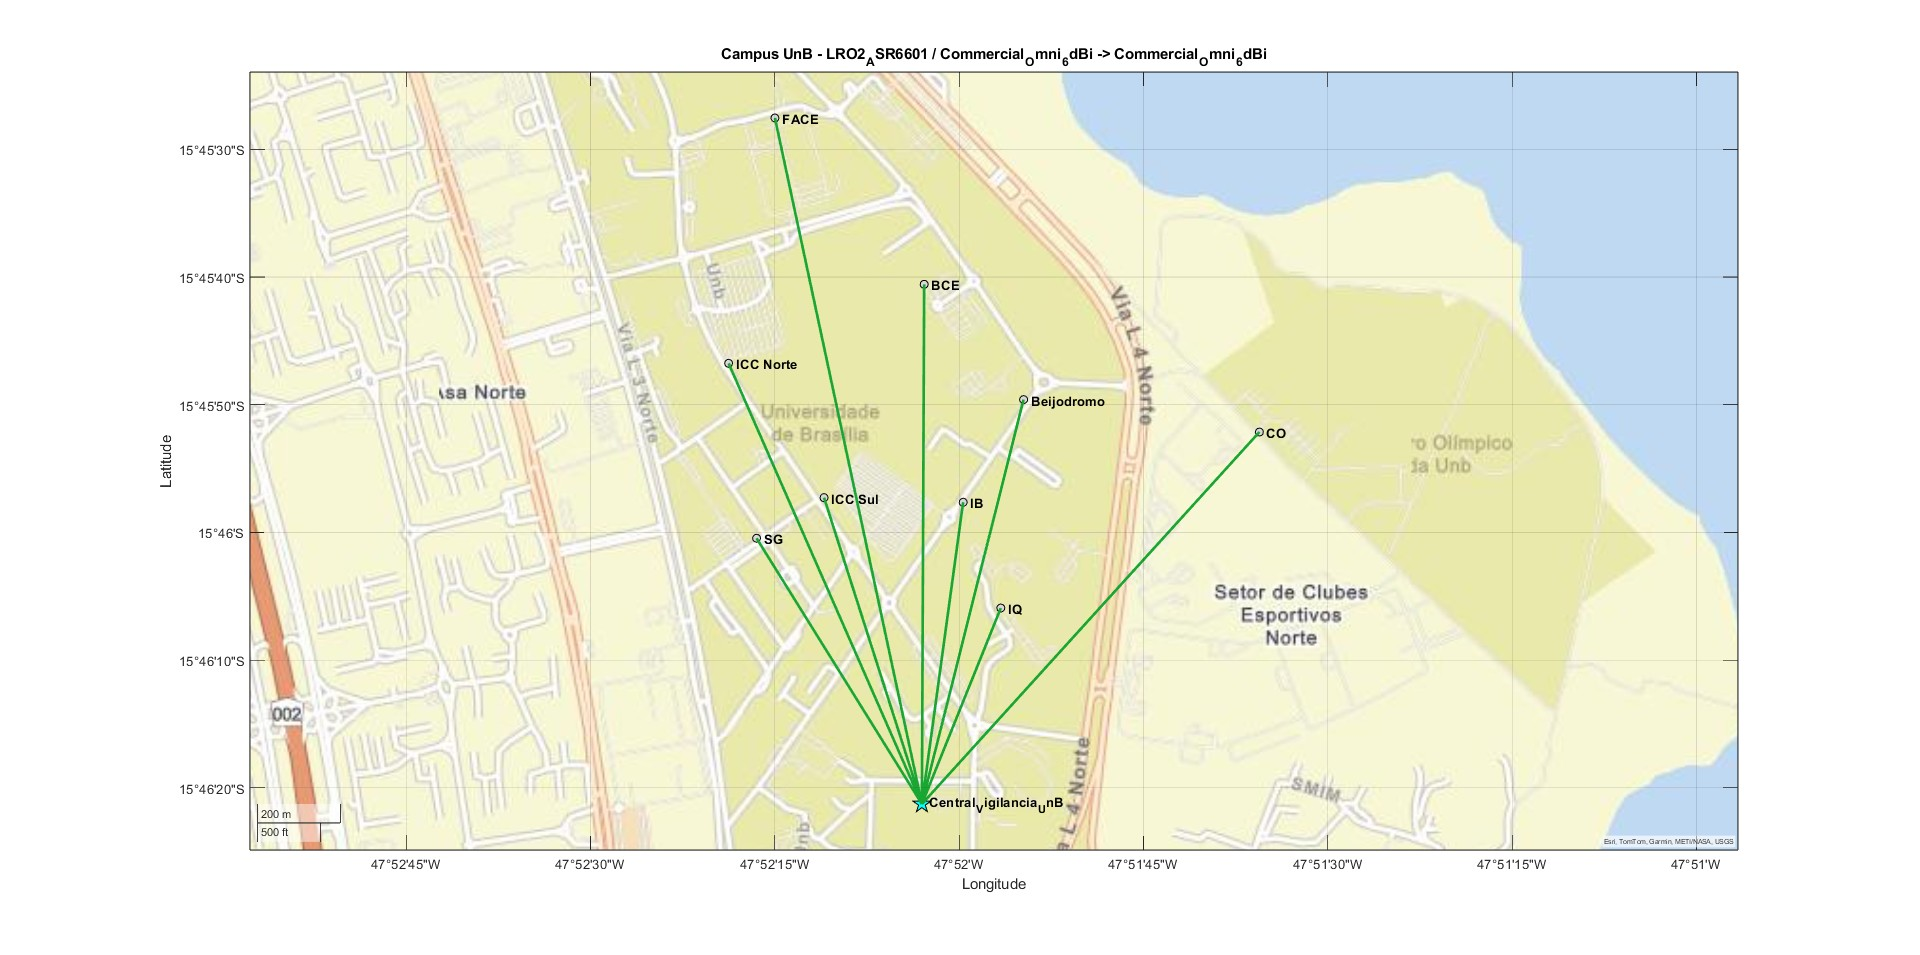
\includegraphics[width=\linewidth,height=0.68\textheight,keepaspectratio]{CampusUnBArranjoMapaSatelite.jpg}
\techcaption{O mapa organiza os pontos de alarme no campus e destaca a lógica de comunicação em estrela: múltiplos nós transmitem para a central/gateway.}
\column{0.38\textwidth}
\vspace{-.5cm}
\small
\begin{block}{Cadeia funcional}
\begin{enumerate}
  \item Botão de segurança.
  \item Módulo LoRa.
  \item Antena do nó.
  \item Propagação no campus.
  \item Antena do gateway.
  \item Central de segurança.
\end{enumerate}
\end{block}
\begin{block}{Consequência}
O gateway recebe sinais de vários azimutes; por isso, cobertura angular é tão importante quanto ganho máximo.
\end{block}
\end{columns}
\end{frame}

% 6
\begin{frame}{Pontos geográficos do Campus Darcy Ribeiro}
\small
\begin{columns}[T,onlytextwidth]
\column{0.50\textwidth}
\begin{table}
\centering
\scriptsize
\begin{tabular}{lrr}
\toprule
Ponto & Latitude & Longitude \\
\midrule
FACE & -15.757651 & -47.870831 \\
BCE & -15.761270 & -47.867457 \\
Beijódromo & -15.763777 & -47.865210 \\
IB & -15.766011 & -47.866576 \\
IQ & -15.768312 & -47.865725 \\
ICC Sul & -15.765911 & -47.869720 \\
ICC Norte & -15.762989 & -47.871878 \\
CO & -15.764482 & -47.859879 \\
SG & -15.766793 & -47.871246 \\
\bottomrule
\end{tabular}
\end{table}
\column{0.46\textwidth}
\centering
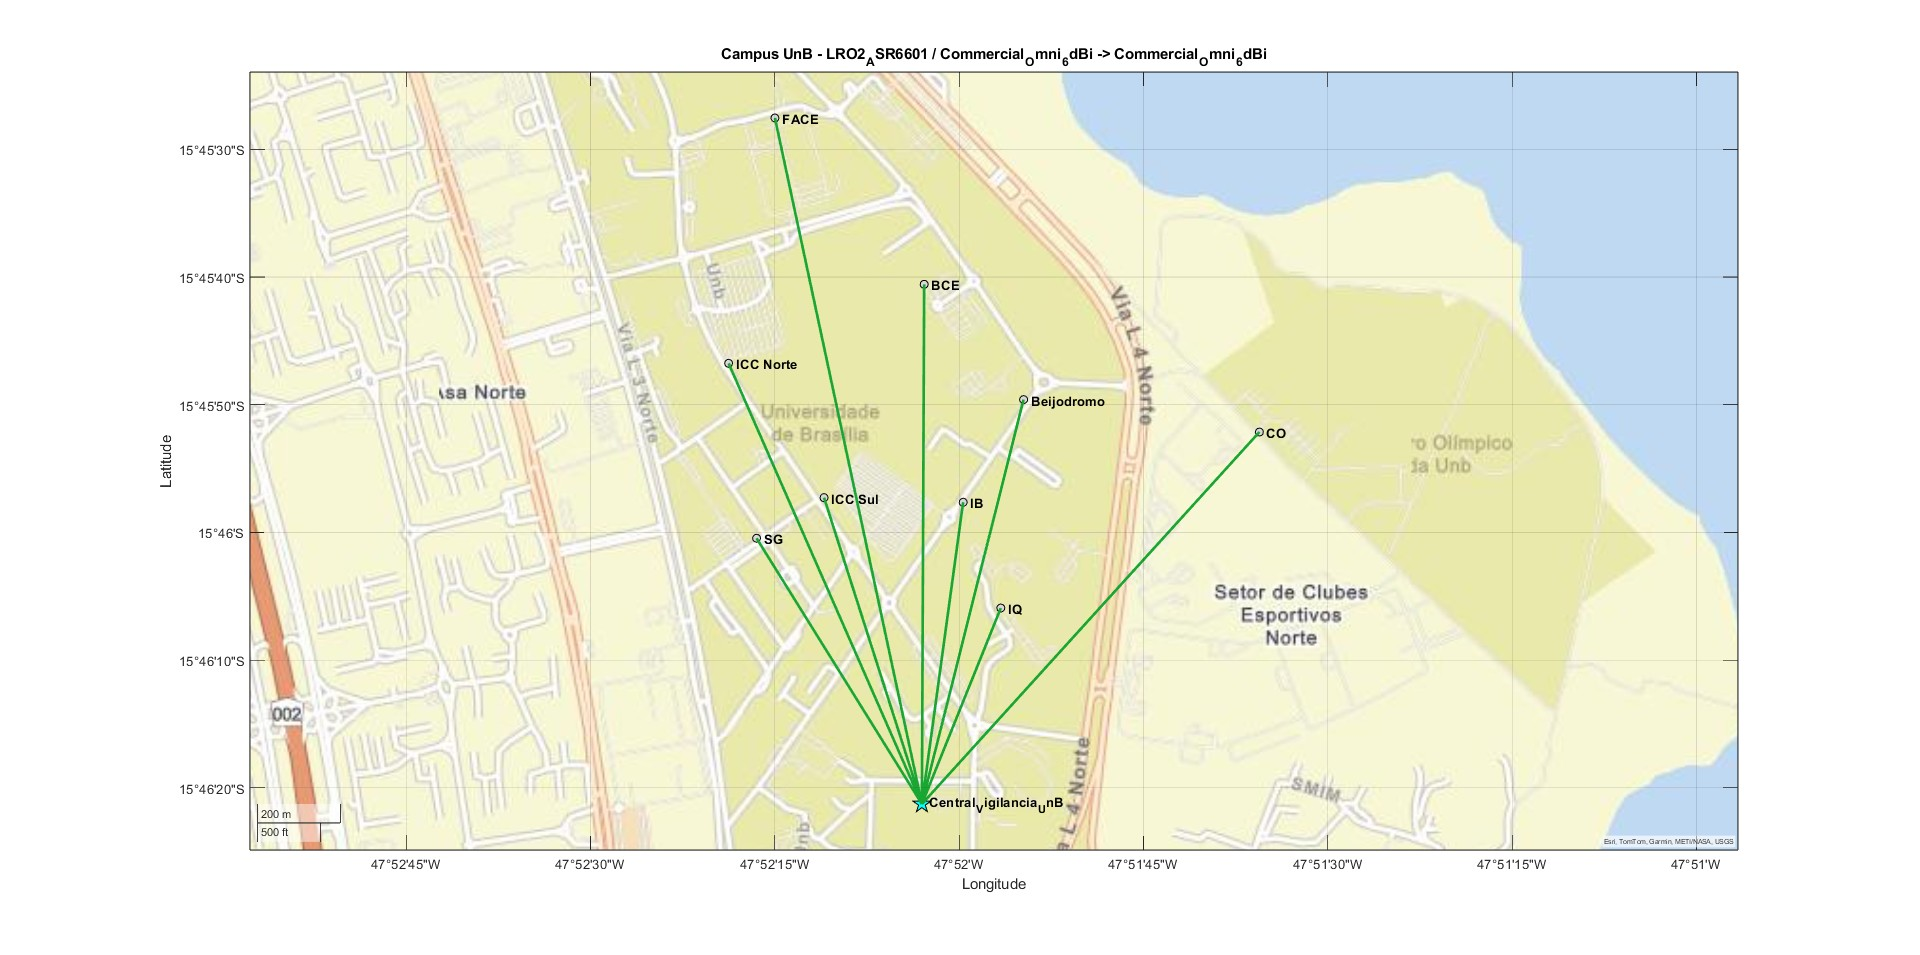
\includegraphics[width=\linewidth,height=0.54\textheight,keepaspectratio]{CampusUnBArranjoMapaSatelite.jpg}
\techcaption{A distribuição espacial produz enlaces com distâncias e azimutes diferentes; a antena deve ser avaliada nessa geometria real.}
\end{columns}
\end{frame}

% 7
\begin{frame}{Escolha do gateway: infraestrutura, não apenas geometria}
\small
\begin{columns}[T,onlytextwidth]
\column{0.50\textwidth}
\begin{block}{Critério de engenharia}
\begin{itemize}
  \item A simulação pode ranquear candidatos por distância média e distância máxima.
  \item Porém, a escolha real é condicionada pela infraestrutura existente da segurança da UnB.
  \item Aproveitar central já instalada reduz custo, tempo de implantação e integração operacional.
\end{itemize}
\end{block}
\column{0.46\textwidth}
\begin{table}
\centering
\scriptsize
\begin{tabular}{lrr}
\toprule
Candidato & Dist. média (m) & Dist. máx. (m) \\
\midrule
IB & 545.61 & 1031.5 \\
ICC Sul & 565.55 & 1066.6 \\
Beijódromo & 578.80 & 907.06 \\
BCE & 617.75 & 886.56 \\
Central Vigilância & 1010.00 & 1689.7 \\
\bottomrule
\end{tabular}
\end{table}
\techcaption{A Central de Vigilância não é a melhor por métrica geométrica, mas é coerente por custo, recursos e integração com a operação existente.}
\end{columns}
\end{frame}

% 8
\begin{frame}{Por que comparar antenas?}
\small
\begin{columns}[T,onlytextwidth]
\column{0.47\textwidth}
\begin{block}{Armadilha comum}
Escolher a antena apenas pelo maior ganho máximo de catálogo ignora a direção do enlace, os nulos do padrão e o papel da antena no sistema.
\end{block}
\begin{block}{Pergunta correta}
Qual antena entrega margem suficiente, instalação viável e cobertura angular adequada para cada função?
\end{block}
\column{0.49\textwidth}
\centering
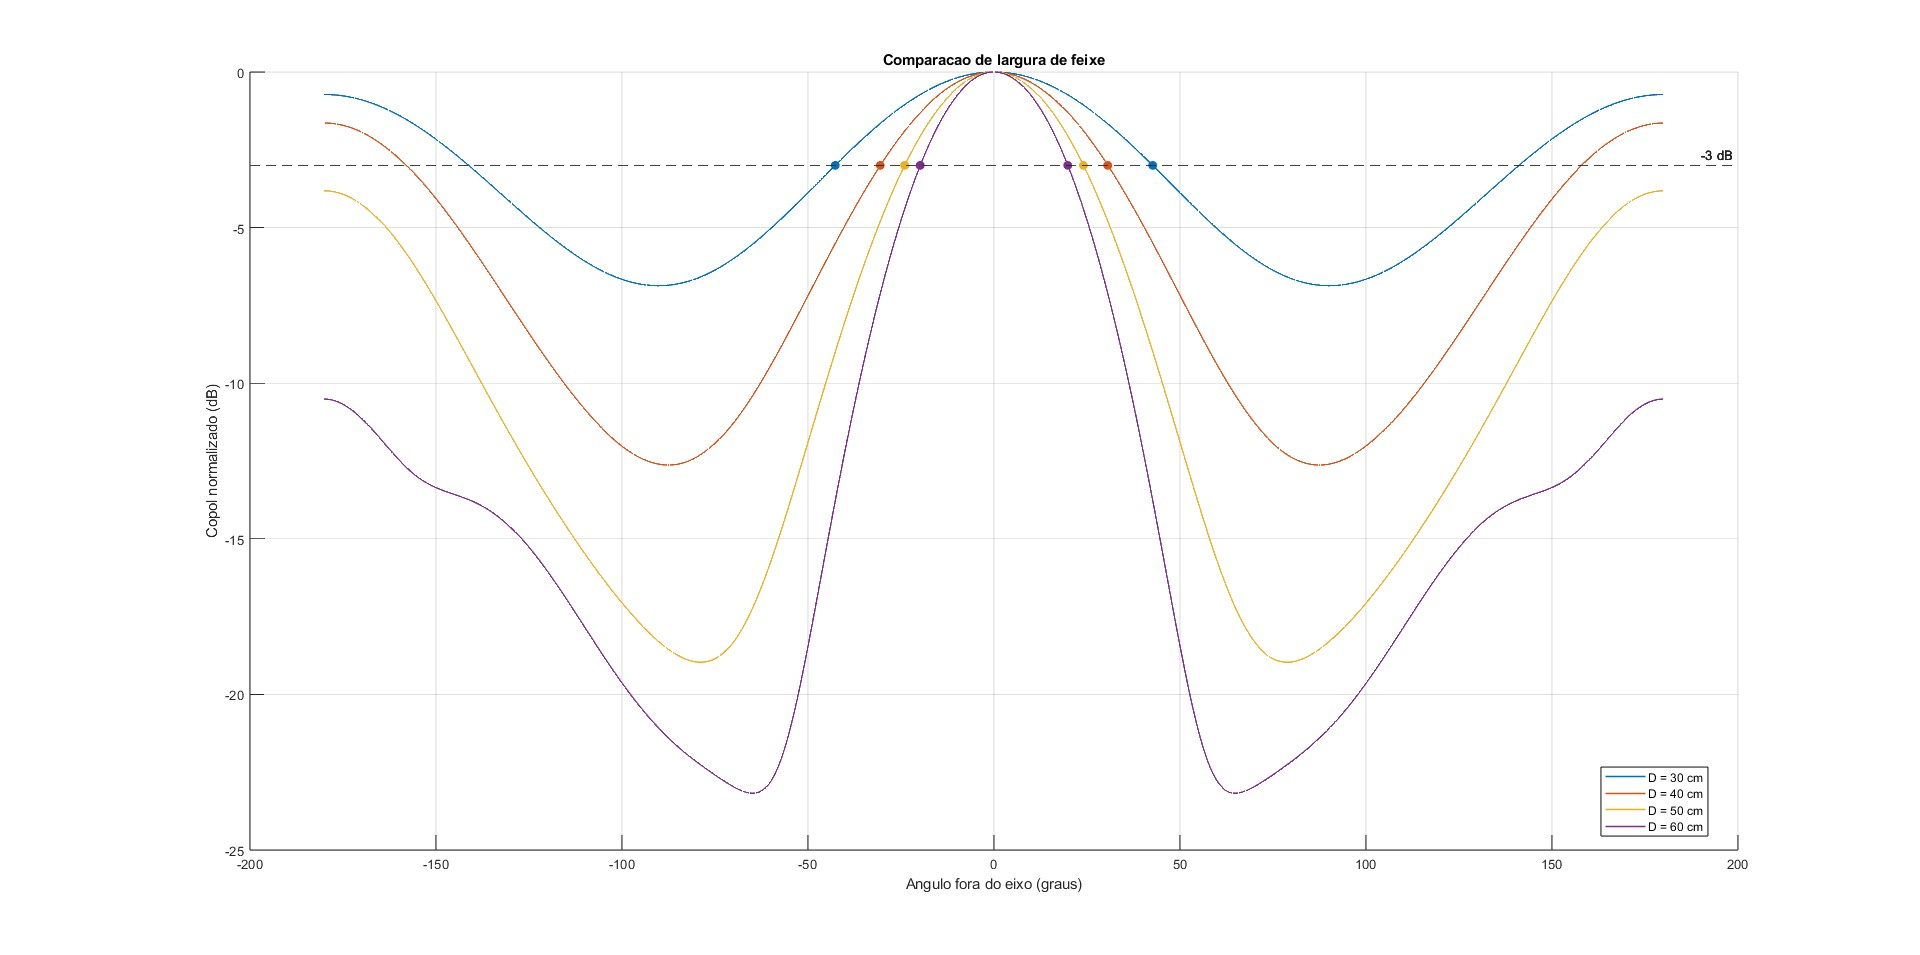
\includegraphics[width=\linewidth,height=0.55\textheight,keepaspectratio]{ComparacaoLarguraDeFeixe.jpg}
\techcaption{O aumento de ganho diretivo geralmente estreita a largura de feixe; o benefício em um enlace apontado pode virar penalidade em recepção multi-azimute.}
\end{columns}
\end{frame}

% 9
\begin{frame}{Parâmetros de antenas usados na análise}
\small
\begin{table}
\centering
\scriptsize
\begin{tabular}{p{0.20\linewidth}p{0.72\linewidth}}
\toprule
Parâmetro & Papel no projeto \\
\midrule
Ganho & Soma potência efetiva na direção desejada; deve ser usado como ganho efetivo, não apenas máximo. \\
Diretividade & Define se a antena cobre muitos azimutes ou concentra energia em um boresight. \\
Polarização & Nós e gateway devem manter polarização compatível; a referência prática é vertical. \\
Largura de banda & A antena precisa operar na faixa LoRa considerada, em torno de \SI{915}{MHz}. \\
$S_{11}$ & Indica casamento de impedância; valores mais negativos tendem a reduzir potência refletida. \\
Largura de feixe & Controla tolerância a apontamento e região angular de cobertura. \\
\bottomrule
\end{tabular}
\end{table}
\begin{block}{Leitura de engenharia}
Para gateway central, a abertura angular pesa muito. Para nós fixos e apontáveis, diretividade pode ser explorada, desde que a instalação suporte alinhamento.
\end{block}
\end{frame}

% 10
\begin{frame}{Modelo de enlace}
\small
\begin{block}{Potência recebida}
\[
P_{rx,\mathrm{dBm}} =
P_{tx,\mathrm{dBm}} + G_{tx,\mathrm{dBi}} + G_{rx,\mathrm{dBi}}
- FSPL_{\mathrm{dB}} - L_{\mathrm{adicionais}}
\]
\end{block}
\begin{block}{Perda em espaço livre}
\[
FSPL_{\mathrm{dB}} = 32{,}44 + 20\log_{10}(f_{\mathrm{MHz}}) + 20\log_{10}(d_{\mathrm{km}})
\]
\end{block}
\begin{block}{Margem de enlace}
\[
M_{\mathrm{dB}} = P_{rx,\mathrm{dBm}} - S_{\mathrm{rx,dBm}}
\]
\end{block}
\end{frame}

% 11
\begin{frame}{Geometria do enlace}
\small
\begin{columns}[T,onlytextwidth]
\column{0.48\textwidth}
\begin{block}{Do mapa ao cálculo}
\begin{itemize}
  \item Coordenadas geográficas são convertidas para um sistema local ENU.
  \item O gateway é usado como origem.
  \item Para cada ponto, calcula-se distância 2D/3D, azimute e elevação.
  \item Para antenas diretivas, calcula-se o ângulo fora do eixo.
\end{itemize}
\end{block}
\column{0.48\textwidth}
\begin{table}
\centering
\scriptsize
\begin{tabular}{lrr}
\toprule
Ponto & Azimute p/ GW & Elevação \\
\midrule
FACE & 167.83$^\circ$ & -0.039$^\circ$ \\
BCE & 180.25$^\circ$ & 0.621$^\circ$ \\
IQ & 202.05$^\circ$ & -0.551$^\circ$ \\
CO & 222.39$^\circ$ & 0.504$^\circ$ \\
SG & 147.95$^\circ$ & -1.036$^\circ$ \\
\bottomrule
\end{tabular}
\end{table}
\techcaption{As elevações são pequenas: o campus gera enlaces quase horizontais, favorecendo antenas verticais com máximo próximo ao horizonte.}
\end{columns}
\end{frame}

% 12
\begin{frame}{Ganho efetivo dependente de direção}
\small
\begin{block}{Ideia central}
\[
G_{\mathrm{efetivo}} = G(\theta,\phi)
\quad \text{ou} \quad
G_{\mathrm{efetivo}} = G(\alpha_{\mathrm{fora\ do\ eixo}})
\]
\end{block}
\begin{columns}[T,onlytextwidth]
\column{0.47\textwidth}
\begin{itemize}
  \item Dipolo e monopolo verticais: enlaces horizontais ficam próximos de $\theta=90^\circ$.
  \item Diretivas: o ganho cai quando a direção do enlace se afasta do boresight.
  \item Parabólica: ganho extraído por interpolação das tabelas WebPRAC.
\end{itemize}
\column{0.49\textwidth}
\begin{block}{Consequência prática}
O cálculo usa $G_{tx}$ e $G_{rx}$ efetivos. Isso evita atribuir o ganho máximo da antena para direções onde o padrão tem queda ou nulos.
\end{block}
\end{columns}
\end{frame}

% 13
\begin{frame}{Antena dipolo de meia onda}
\begin{columns}[T,onlytextwidth]
\column{0.54\textwidth}
\centering
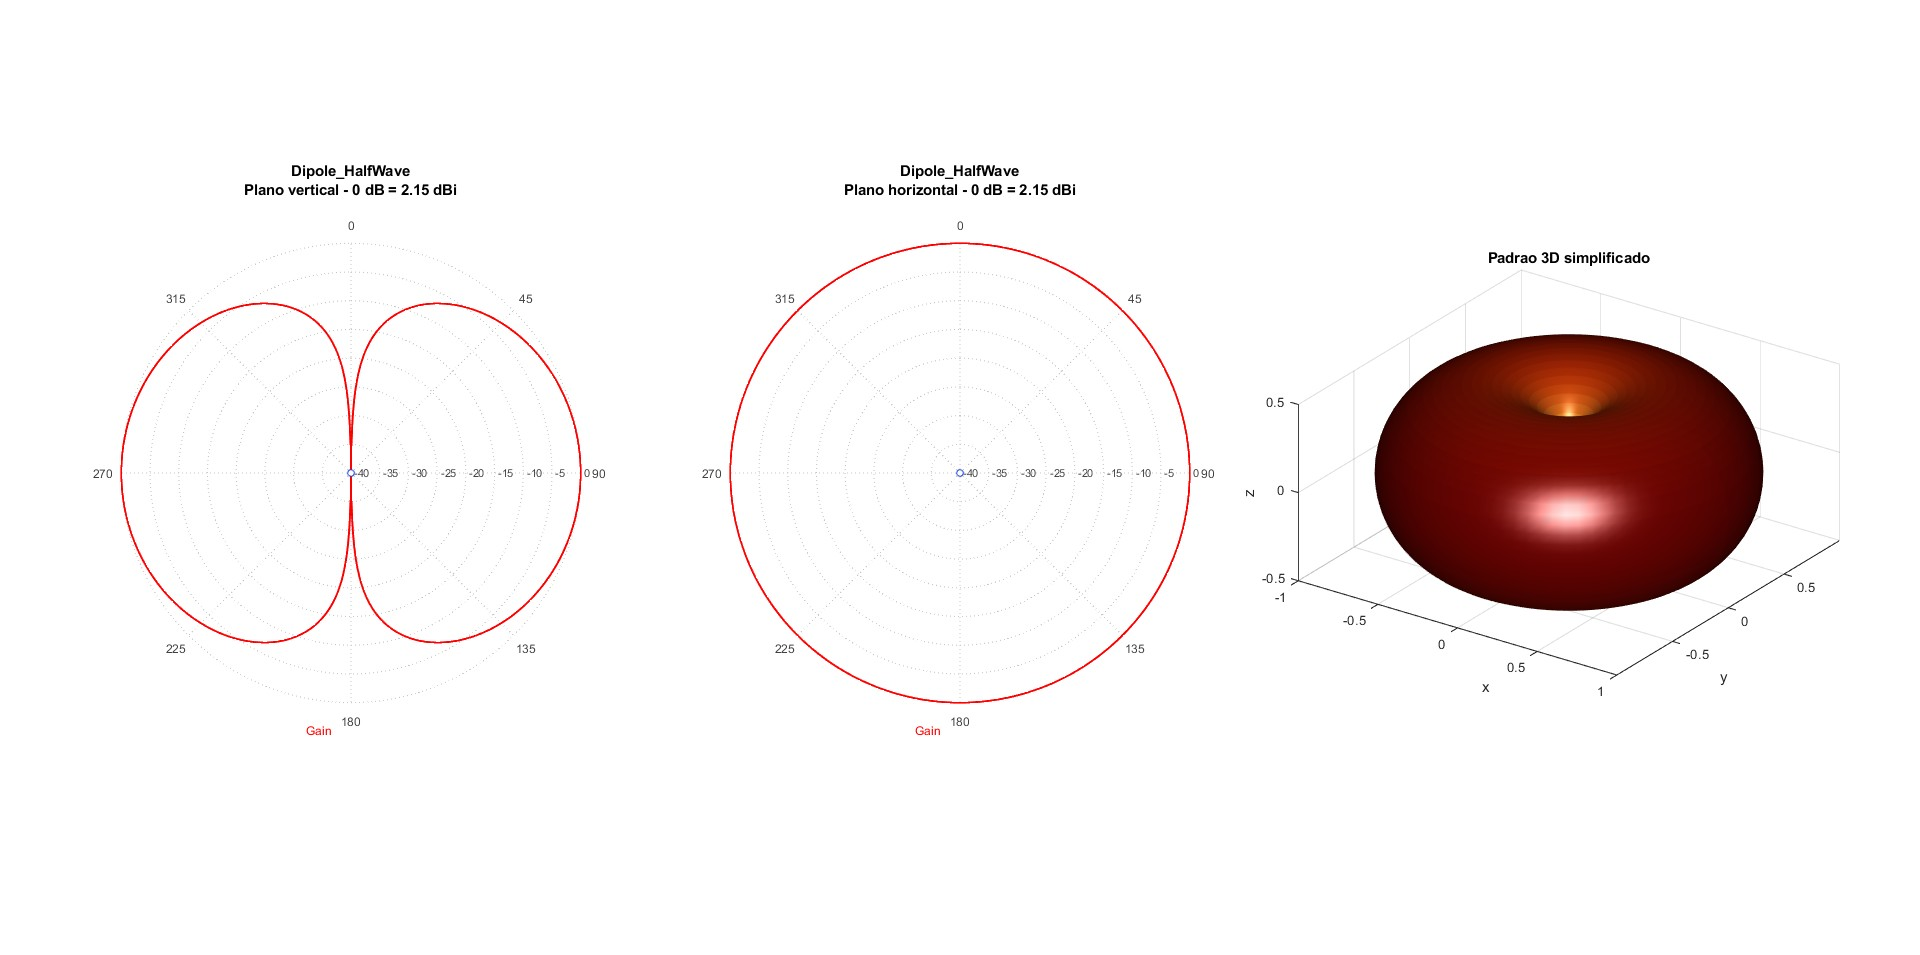
\includegraphics[width=\linewidth,height=0.62\textheight,keepaspectratio]{DipoleHalfWave.jpg}
\techcaption{O dipolo vertical é aproximadamente omnidirecional no plano horizontal e apresenta nulos ao longo do eixo da antena.}
\column{0.42\textwidth}
\small
\begin{itemize}
  \item Ganho máximo de referência: cerca de \SI{2.15}{dBi}.
  \item Bom ponto de comparação teórica.
  \item Simples, barato e fisicamente viável.
  \item Adequado a nós ou gateway quando se deseja cobertura horizontal ampla.
  \item Cuidados: montagem vertical, polarização e afastamento de estruturas metálicas.
\end{itemize}
\end{columns}
\end{frame}

% 14
\begin{frame}{Antena monopolo sobre plano de terra}
\begin{columns}[T,onlytextwidth]
\column{0.54\textwidth}
\centering
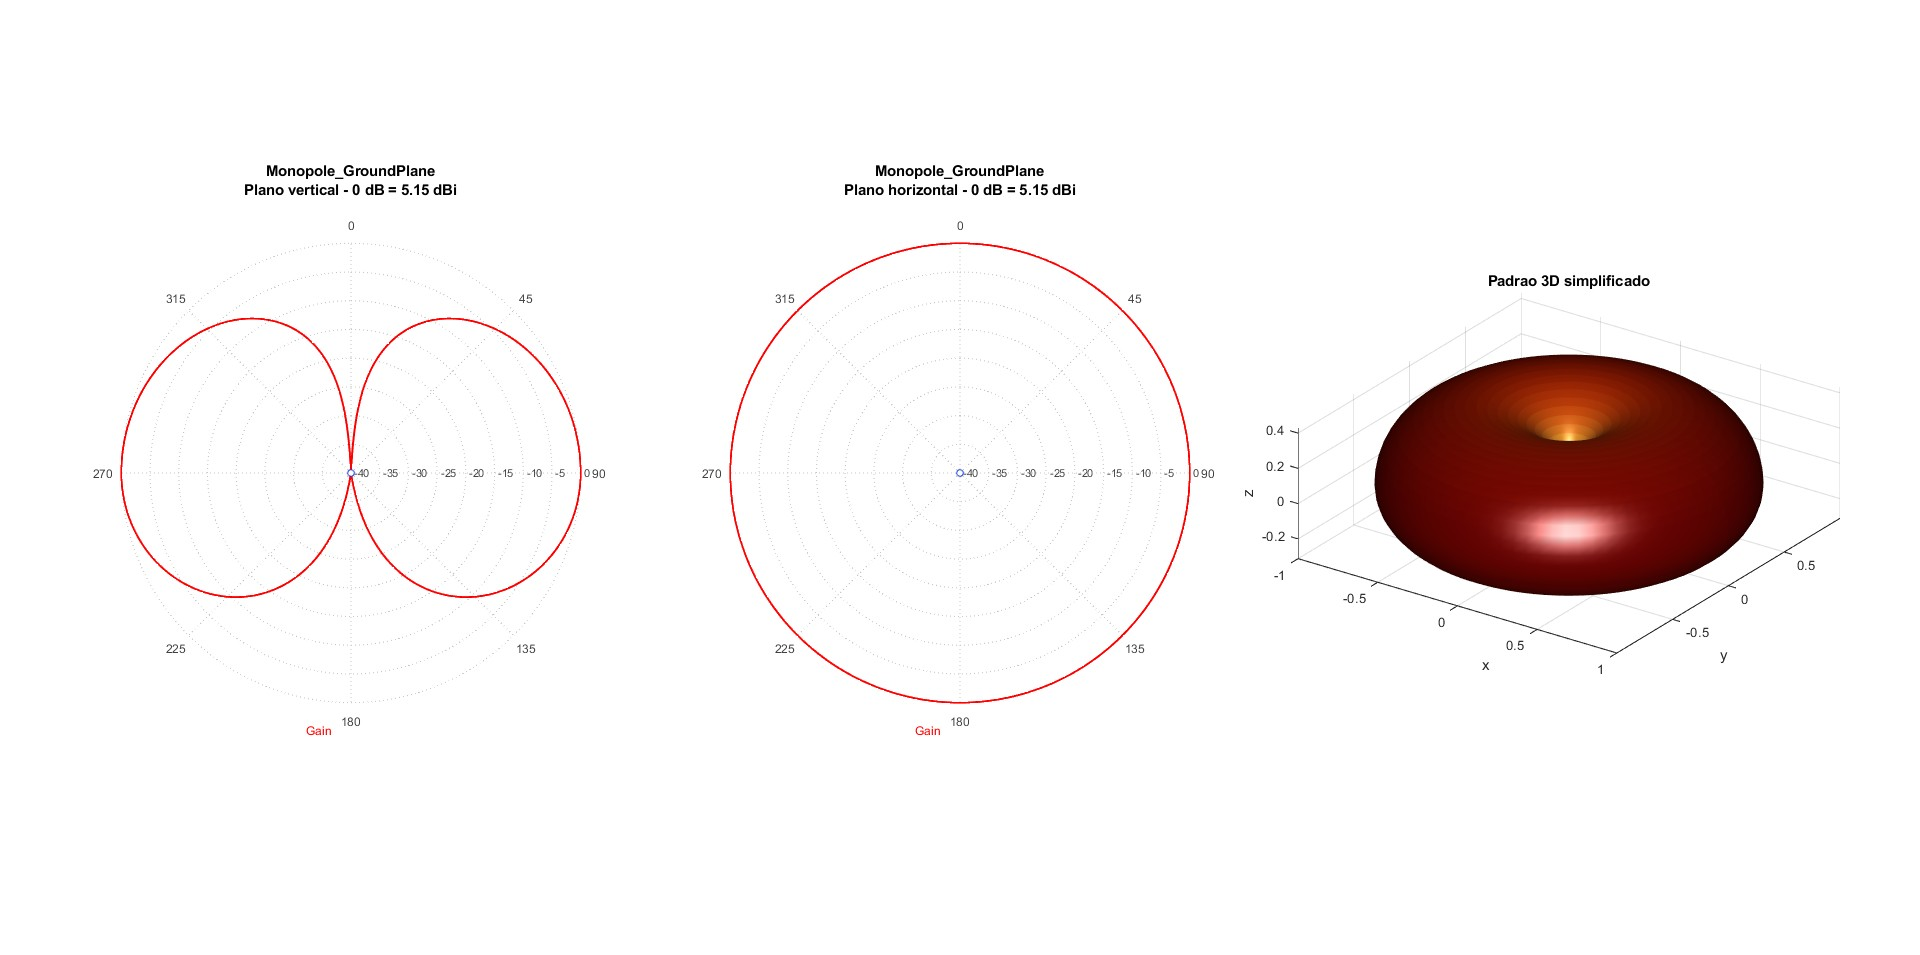
\includegraphics[width=\linewidth,height=0.62\textheight,keepaspectratio]{MonopoleGroundPlane.jpg}
\techcaption{O monopolo concentra radiação próxima ao horizonte no semiespaço superior; por isso combina bem com enlaces quase horizontais no campus.}
\column{0.42\textwidth}
\small
\begin{itemize}
  \item Ganho ideal de referência: cerca de \SI{5.15}{dBi}.
  \item Polarização vertical.
  \item Instalação prática em postes, caixas e mastros.
  \item Exige plano de terra ou radiais adequados.
  \item Forte candidato para nós de alarme por simplicidade e cobertura horizontal.
\end{itemize}
\end{columns}
\end{frame}

% 15
\begin{frame}{Antena helicoidal axial}
\begin{columns}[T,onlytextwidth]
\column{0.54\textwidth}
\centering
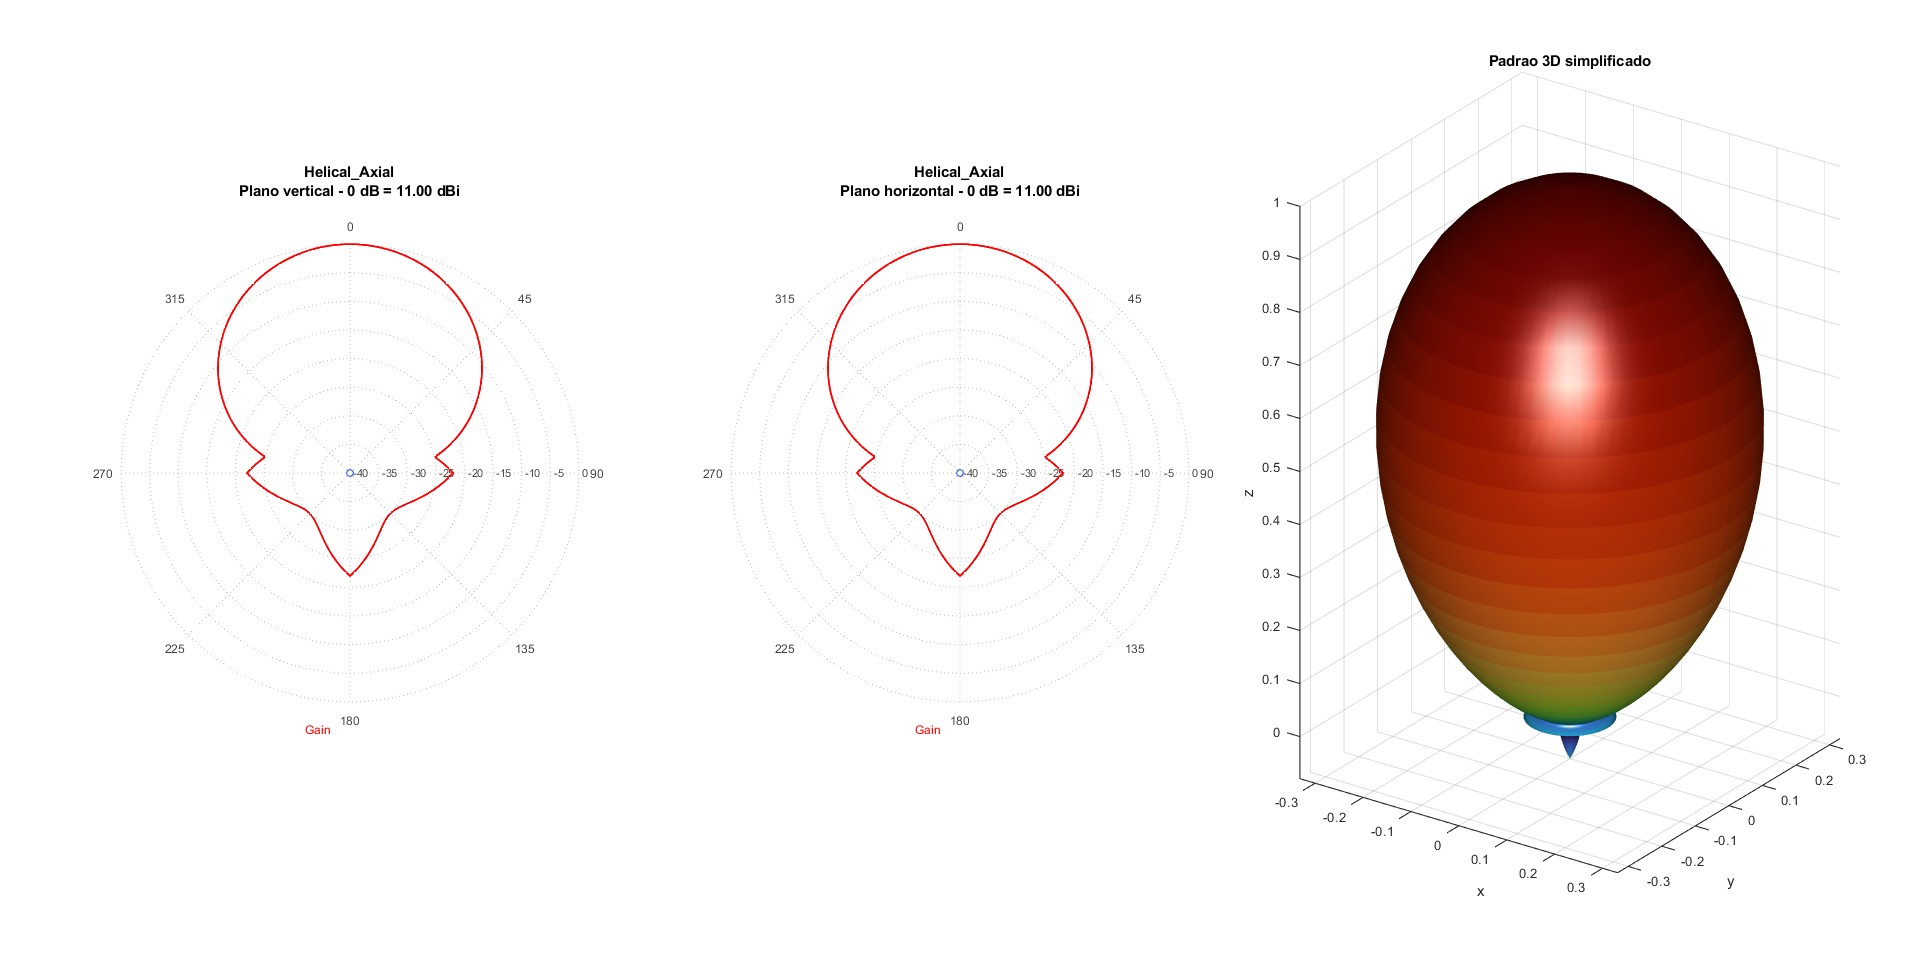
\includegraphics[width=\linewidth,height=0.62\textheight,keepaspectratio]{Helicoidal.jpg}
\techcaption{A helicoidal é mais diretiva que dipolo/monopolo: o máximo fica no boresight e a largura de feixe define a tolerância de apontamento.}
\column{0.42\textwidth}
\small
\begin{itemize}
  \item Pode aumentar margem em enlace fixo apontado.
  \item Não é naturalmente adequada como antena única de gateway central.
  \item Exige orientação mecânica estável.
  \item Deve ser avaliada com polarização e alinhamento coerentes.
  \item Útil como comparação entre soluções omni e diretivas.
\end{itemize}
\end{columns}
\end{frame}

% 16
\begin{frame}{Antena PCB compacta}
\begin{columns}[T,onlytextwidth]
\column{0.54\textwidth}
\centering
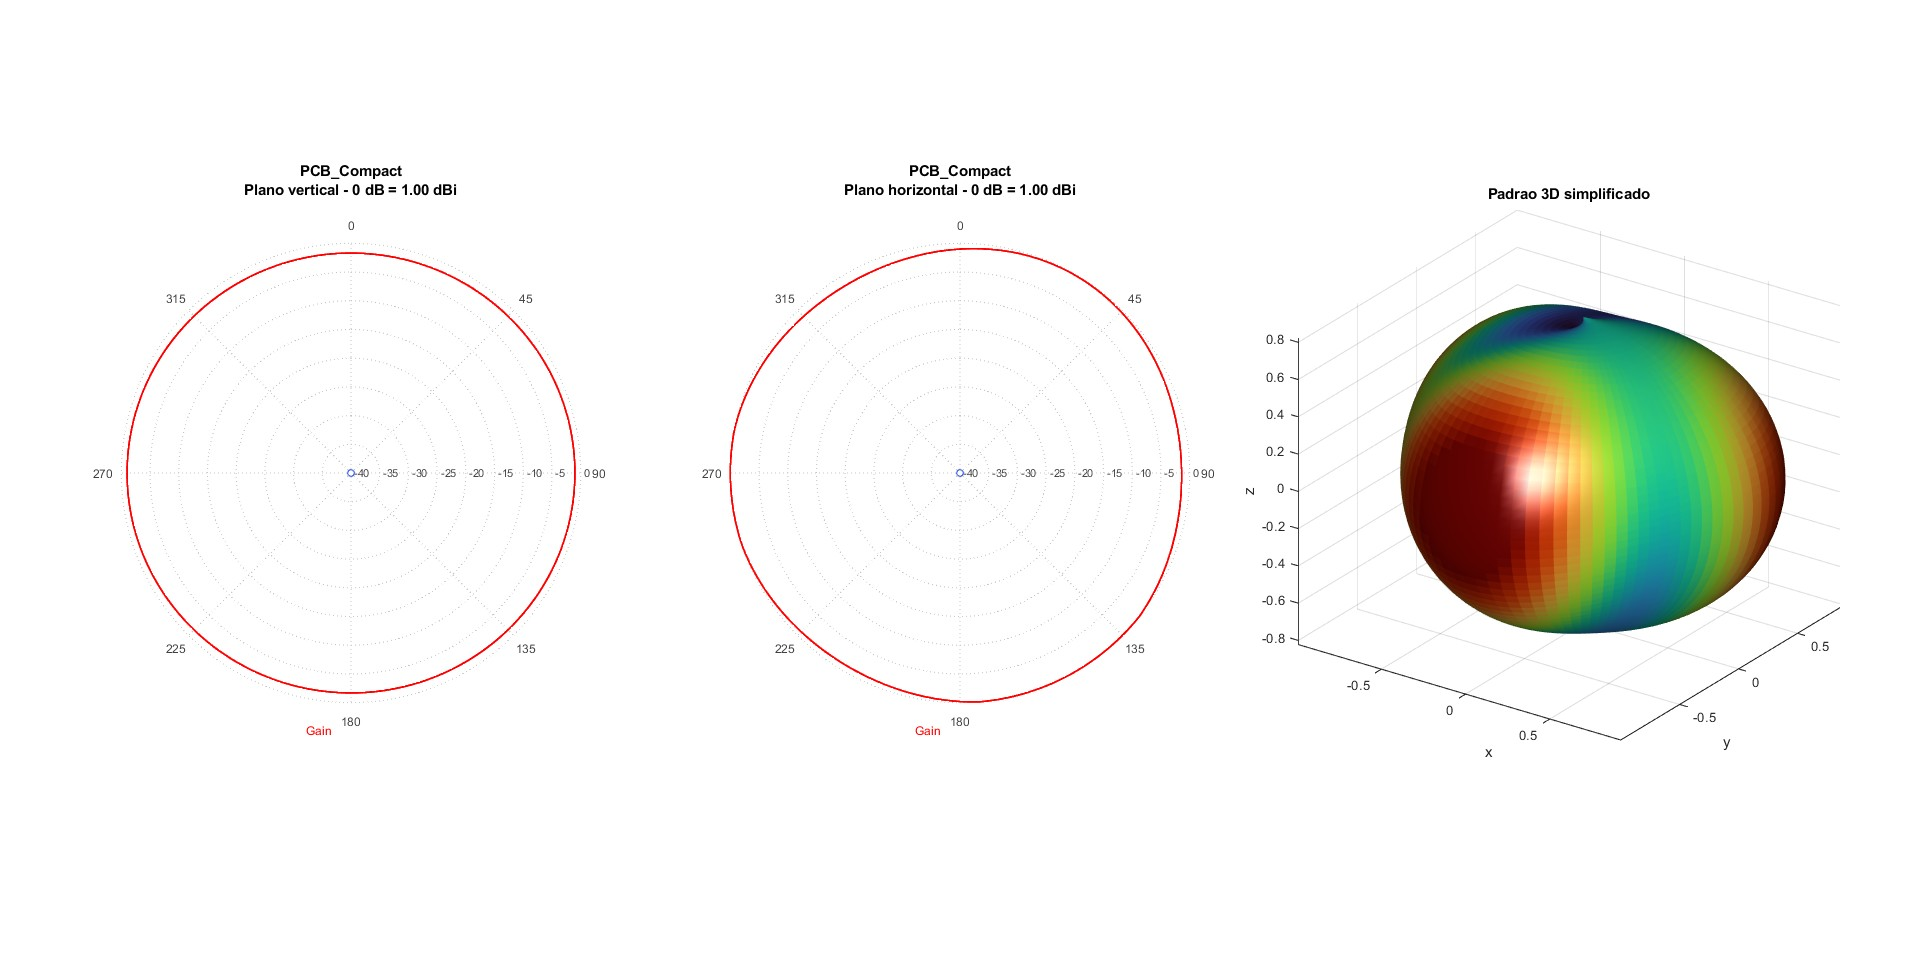
\includegraphics[width=\linewidth,height=0.62\textheight,keepaspectratio]{PCBcompacta.jpg}
\techcaption{A antena PCB facilita integração e custo, mas o padrão tende a ser menos controlado e mais dependente da placa, caixa e instalação.}
\column{0.42\textwidth}
\small
\begin{itemize}
  \item Solução compacta e barata para nós de alarme.
  \item Menor volume mecânico e instalação discreta.
  \item Normalmente menor ganho que antenas externas.
  \item Desempenho sensível ao layout, plano de terra e encapsulamento.
  \item Boa candidata quando custo e integração dominam a decisão.
\end{itemize}
\end{columns}
\end{frame}

% 17
\begin{frame}{Antena comercial omnidirecional vertical de 6 dBi}
\begin{columns}[T,onlytextwidth]
\column{0.54\textwidth}
\centering
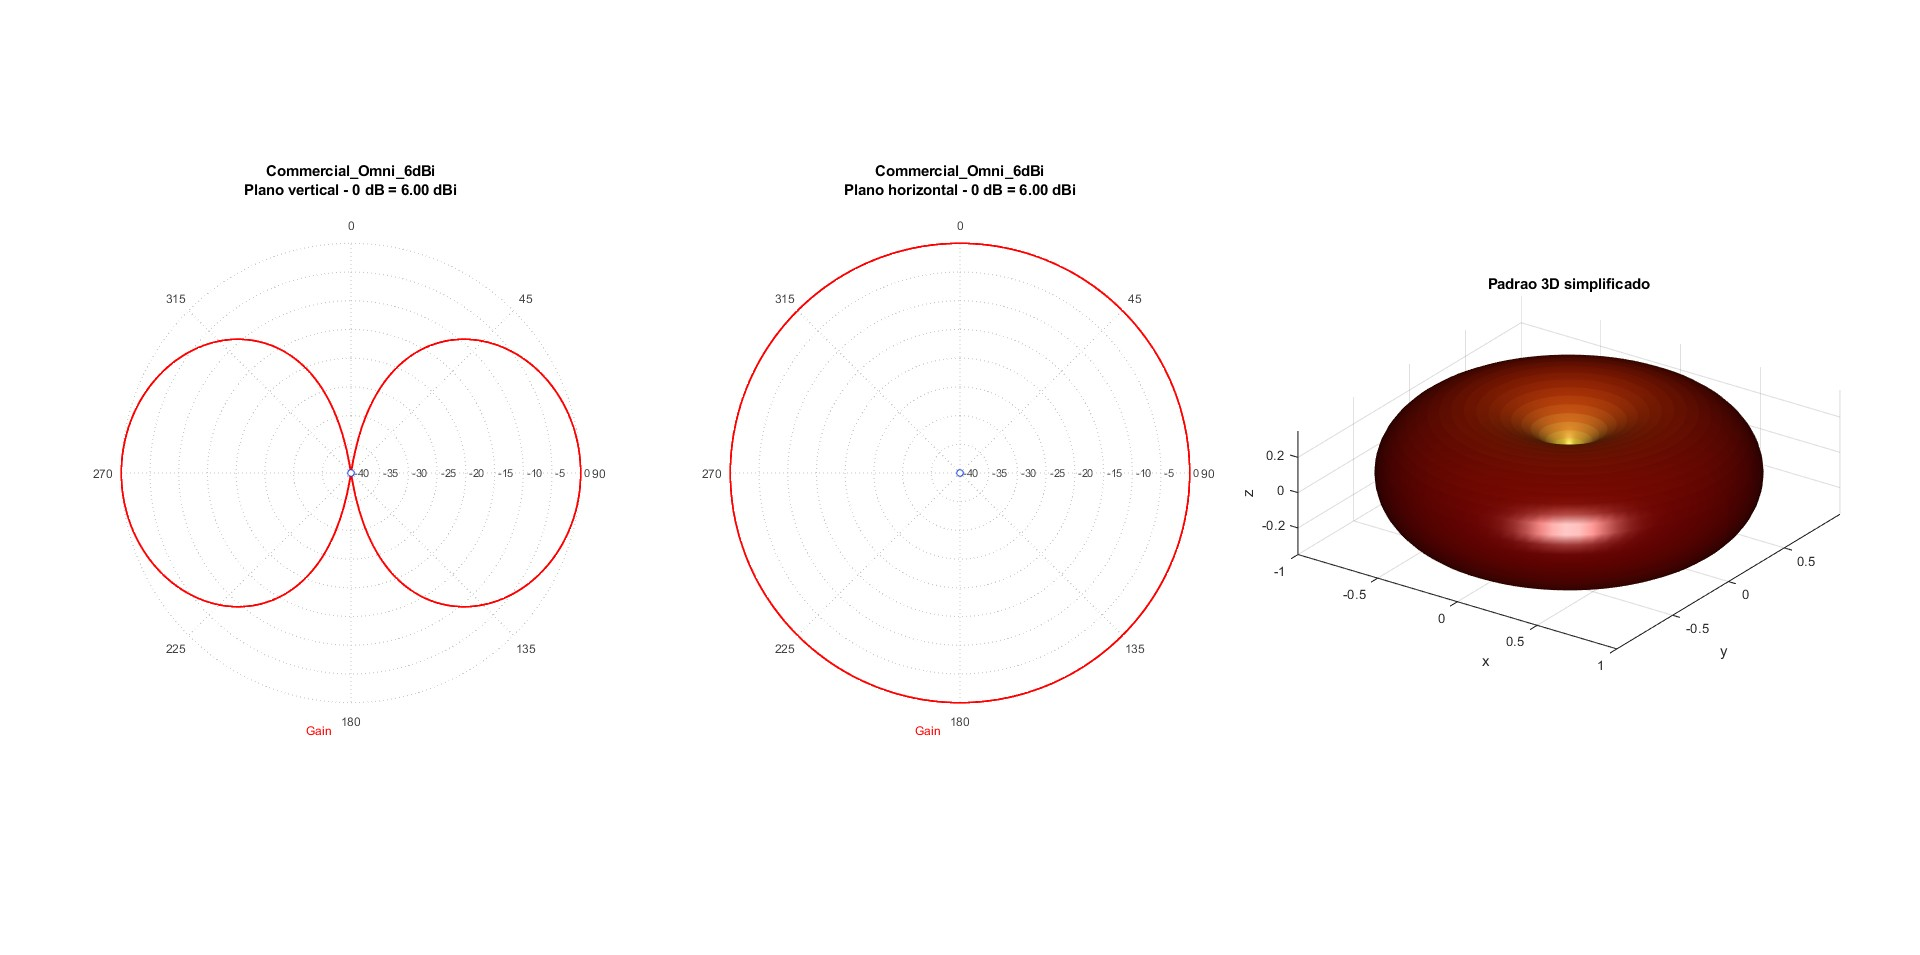
\includegraphics[width=\linewidth,height=0.62\textheight,keepaspectratio]{ComercialOmni6dBi.jpg}
\techcaption{A antena comercial 868/915 MHz fornece referência prática: polarização vertical, conectorização pronta e cobertura horizontal em múltiplas direções.}
\column{0.42\textwidth}
\small
\begin{itemize}
  \item Ganho nominal: \SI{6}{dBi}.
  \item Solução pronta para implantação com módulos LoRa.
  \item Excelente coerência para gateway central único.
  \item Também é prática para nós quando há espaço físico.
  \item Ranking agregado da simulação apontou esta opção como a mais forte para gateway e nós.
\end{itemize}
\end{columns}
\end{frame}

% 18
\begin{frame}{Antena parabólica}
\begin{columns}[T,onlytextwidth]
\column{0.54\textwidth}
\centering
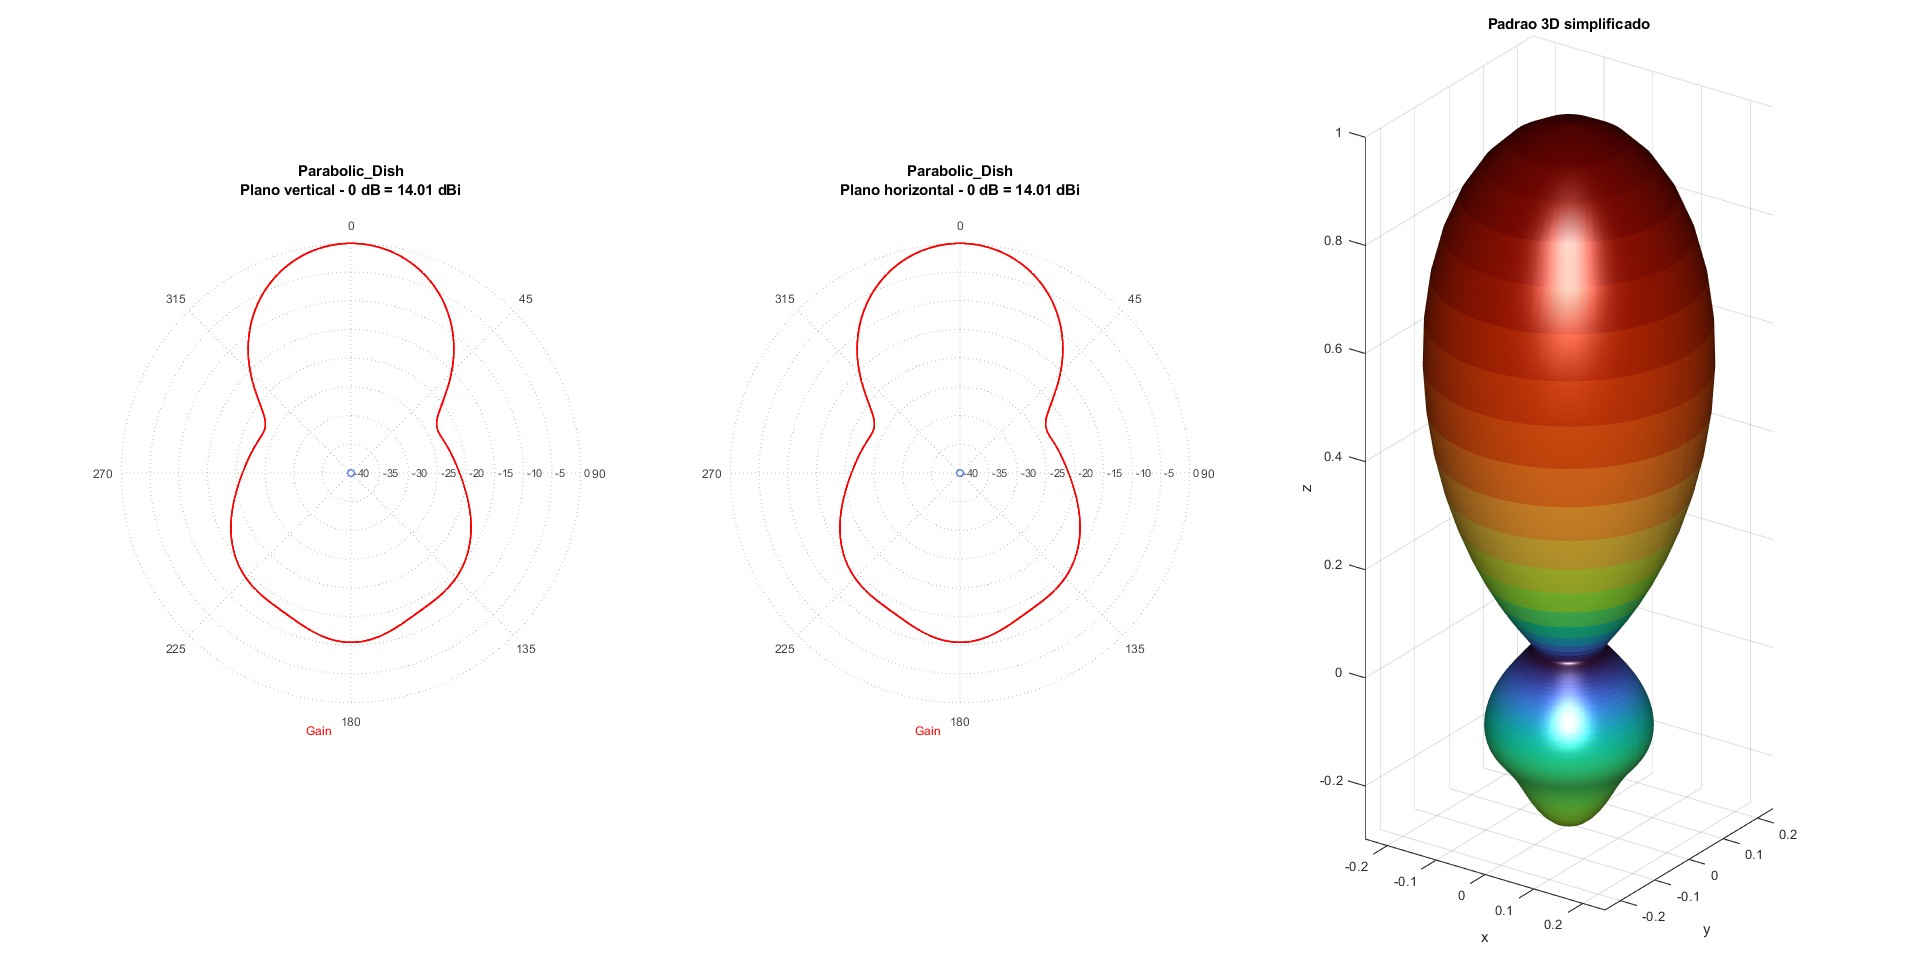
\includegraphics[width=\linewidth,height=0.62\textheight,keepaspectratio]{Parabolica14dBi.jpg}
\techcaption{A parabólica concentra energia em um feixe estreito: útil para enlace fixo apontado, ruim como antena única recebendo de vários azimutes.}
\column{0.42\textwidth}
\small
\begin{itemize}
  \item Maior ganho quando bem apontada.
  \item Ganho cai rapidamente fora do eixo principal.
  \item Exige suporte mecânico, alinhamento e resistência a vento.
  \item Boa para estudar o limite de ganho diretivo.
  \item Não deve ser apresentada como melhor solução geral do sistema.
\end{itemize}
\end{columns}
\end{frame}

% 19
\begin{frame}{Parabólica: limite prático de $D \leq \SI{60}{cm}$}
\small
\begin{block}{Por que limitar o diâmetro?}
O limite de $D \leq \SI{60}{cm}$ foi imposto por viabilidade prática em postes e instalações externas do campus.
\end{block}
\begin{columns}[T,onlytextwidth]
\column{0.48\textwidth}
\begin{itemize}
  \item Antenas maiores ficam mais pesadas.
  \item Exigem estrutura mecânica mais robusta.
  \item Precisam de alinhamento mais preciso.
  \item Sofrem mais com vento, chuva e tempestades.
\end{itemize}
\column{0.48\textwidth}
\begin{itemize}
  \item Aumentam custo de instalação e manutenção.
  \item Tornam a solução menos discreta.
  \item Podem ser inviáveis para múltiplos pontos.
  \item Fazem sentido apenas quando o ganho adicional justifica a complexidade.
\end{itemize}
\end{columns}
\end{frame}

% 20
\begin{frame}{Parabólicas pequenas: $D=30$, 40, 50 e \SI{60}{cm}}
\small
\begin{table}
\centering
\begin{tabular}{rrrrr}
\toprule
$D$ (cm) & $G_{\max}$ PRAC (dBi) & HPBW PRAC & $G_{\max}$ analítico & HPBW analítico \\
\midrule
30 & 7.99 & 85.34$^\circ$ & 6.96 & 76.45$^\circ$ \\
40 & 10.49 & 61.15$^\circ$ & 9.46 & 57.34$^\circ$ \\
50 & 12.42 & 48.04$^\circ$ & 11.40 & 45.87$^\circ$ \\
60 & 14.01 & 39.66$^\circ$ & 12.98 & 38.23$^\circ$ \\
\bottomrule
\end{tabular}
\end{table}
\begin{block}{Leitura}
O ganho cresce com o diâmetro, mas a largura de feixe diminui. A margem melhora no eixo, enquanto a tolerância angular e a viabilidade mecânica pioram.
\end{block}
\end{frame}

% 21
\begin{frame}{Uso das tabelas WebPRAC de ganho por ângulo}
\begin{columns}[T,onlytextwidth]
\column{0.54\textwidth}
\centering
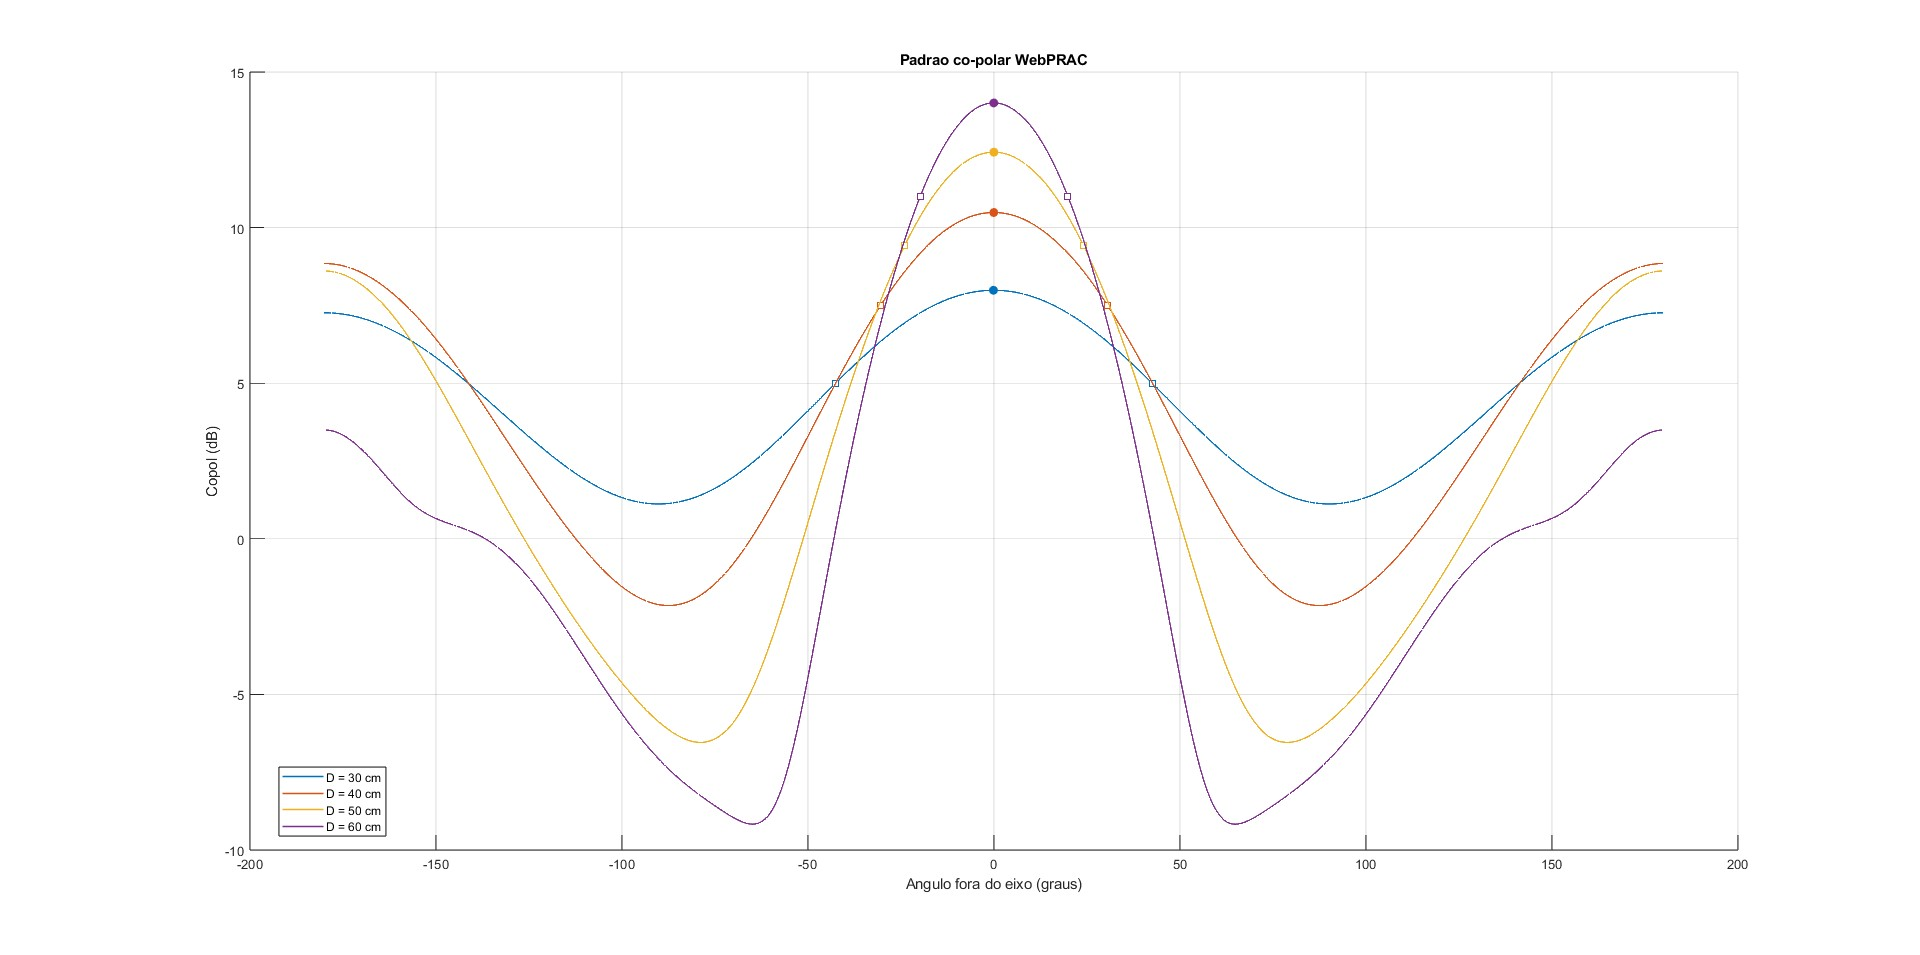
\includegraphics[width=\linewidth,height=0.62\textheight,keepaspectratio]{PadraoCoPolarWebPRAC.jpg}
\techcaption{O WebPRAC fornece ganho co-polar em função do ângulo. A simulação interpola essa curva para obter o ganho efetivo da parabólica.}
\column{0.42\textwidth}
\small
\begin{itemize}
  \item Frequência: \SI{915}{MHz}.
  \item Diâmetros analisados: 30, 40, 50 e \SI{60}{cm}.
  \item Componente usada no enlace: co-polar.
  \item Entrada do cálculo: ângulo fora do eixo.
  \item Saída: $G_{\text{parabólica}}(\alpha)$, não ganho máximo constante.
\end{itemize}
\end{columns}
\end{frame}

% 22
\begin{frame}{Trade-off entre ganho e abertura de feixe}
\begin{columns}[T,onlytextwidth]
\column{0.56\textwidth}
\centering
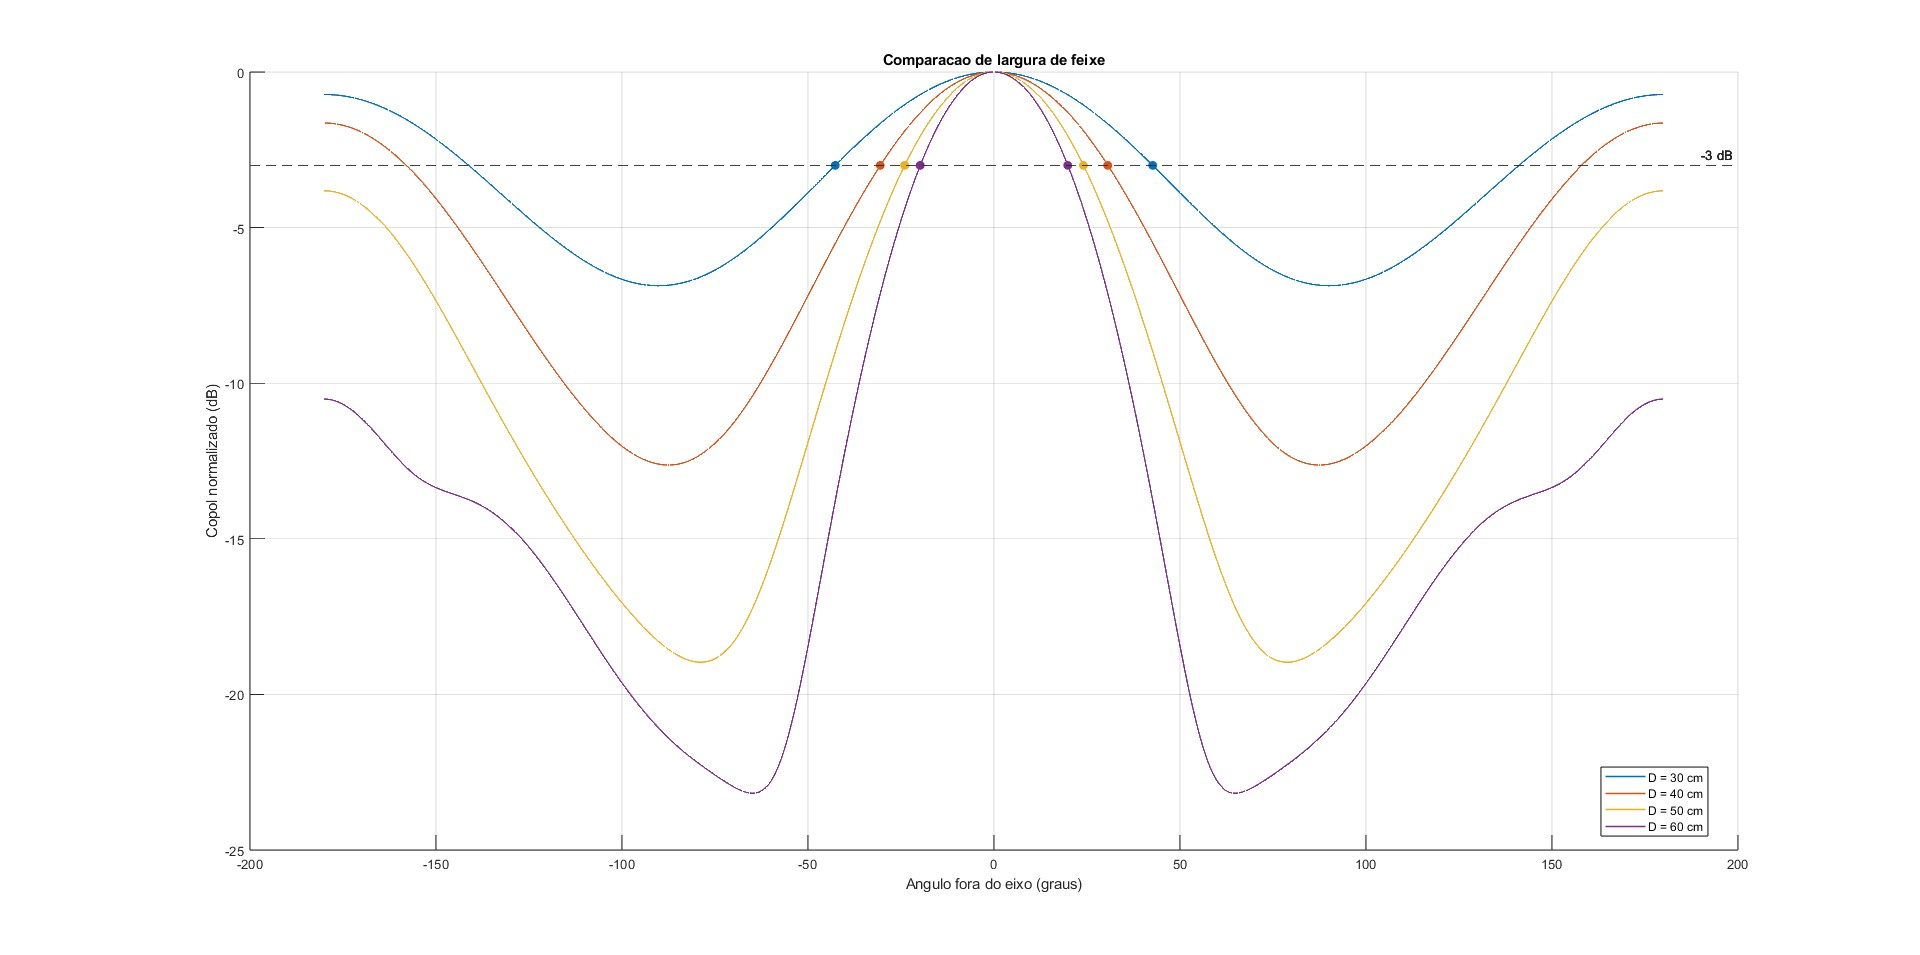
\includegraphics[width=\linewidth,height=0.62\textheight,keepaspectratio]{ComparacaoLarguraDeFeixe.jpg}
\techcaption{Antenas omnidirecionais sacrificam ganho máximo para cobrir azimutes; antenas diretivas aumentam ganho no boresight e reduzem cobertura angular.}
\column{0.40\textwidth}
\small
\begin{block}{Impacto no campus}
\begin{itemize}
  \item Gateway: precisa escutar várias direções.
  \item Nó fixo: pode apontar para a central.
  \item Erro de apontamento vira perda de margem.
  \item Mais ganho não implica mais robustez sistêmica.
\end{itemize}
\end{block}
\end{columns}
\end{frame}

% 23
\begin{frame}{Módulos LoRa comparados}
\small
\begin{table}
\centering
\scriptsize
\begin{tabular}{p{0.22\linewidth}p{0.20\linewidth}p{0.18\linewidth}p{0.27\linewidth}}
\toprule
Módulo & Potência TX & Sensibilidade usada & Observações \\
\midrule
RFM95W 915 MHz & até \SI{20}{dBm} & -139, -136, -118 dBm & Baixo consumo documentado; \SI{120}{mA} em \SI{20}{dBm}. \\
LRO2 ASR6601 & até \SI{22}{dBm} & -138 dBm & Melhor margem agregada na simulação. \\
E220-900T22D & 10 a \SI{22}{dBm} & default ajustável, ex. -137 dBm & Kit associado à antena omni \SI{6}{dBi}; atenção à diferença 100 mW vs. 22 dBm. \\
\bottomrule
\end{tabular}
\end{table}
\begin{block}{Leitura}
O módulo define potência, sensibilidade e consumo; a antena define como essa potência é distribuída no espaço.
\end{block}
\end{frame}

% 24
\begin{frame}{Cálculo de FSPL}
\small
\begin{block}{Exemplo com \SI{915}{MHz}}
\[
FSPL = 32{,}44 + 20\log_{10}(915) + 20\log_{10}(d_{\mathrm{km}})
\]
\end{block}
\begin{table}
\centering
\scriptsize
\begin{tabular}{lrr}
\toprule
Ponto & Distância 3D (m) & FSPL (dB) \\
\midrule
FACE & 1689.7 & 96.225 \\
BCE & 1251.3 & 93.615 \\
Beijódromo & 1004.5 & 91.707 \\
IB & 733.4 & 88.975 \\
IQ & 509.1 & 85.805 \\
ICC Sul & 774.8 & 89.452 \\
ICC Norte & 1159.8 & 92.956 \\
CO & 1212.8 & 93.344 \\
SG & 755.1 & 89.228 \\
\bottomrule
\end{tabular}
\end{table}
\end{frame}

% 25
\begin{frame}{Cálculo de potência recebida}
\small
\begin{block}{Cenário de referência}
RFM95W, \SI{20}{dBm}, dipolo no nó e no gateway, perdas adicionais de \SI{19}{dB} e sensibilidade de -139 dBm.
\end{block}
\begin{table}
\centering
\scriptsize
\begin{tabular}{lrrrr}
\toprule
Ponto & $G_{tx}$ & $G_{rx}$ & FSPL & $P_{rx}$ (dBm) \\
\midrule
FACE & 2.15 & 2.15 & 96.225 & -90.925 \\
BCE & 2.15 & 2.15 & 93.615 & -88.316 \\
Beijódromo & 2.15 & 2.15 & 91.707 & -86.408 \\
IB & 2.15 & 2.15 & 88.975 & -83.675 \\
IQ & 2.15 & 2.15 & 85.805 & -80.506 \\
ICC Sul & 2.15 & 2.15 & 89.452 & -84.152 \\
ICC Norte & 2.15 & 2.15 & 92.956 & -87.656 \\
CO & 2.15 & 2.15 & 93.344 & -88.045 \\
SG & 2.15 & 2.15 & 89.228 & -83.931 \\
\bottomrule
\end{tabular}
\end{table}
\end{frame}

% 26
\begin{frame}{Cálculo de margem de enlace}
\small
\begin{block}{Classificação adotada}
\begin{itemize}
  \item Falha: margem $< \SI{0}{dB}$.
  \item Crítico: $0 \leq$ margem $< \SI{10}{dB}$.
  \item Confortável: margem $\geq \SI{10}{dB}$.
\end{itemize}
\end{block}
\begin{block}{Exemplo}
Para FACE no cenário de referência:
\[
M = -90{,}925 - (-139) = \SI{48.075}{dB}
\]
Mesmo o ponto mais distante fica confortável nesse cenário, antes de discutir custo, instalação e robustez.
\end{block}
\end{frame}

% 27
\begin{frame}{Tabela de pontos e distâncias}
\small
\begin{table}
\centering
\scriptsize
\begin{tabular}{lrrr}
\toprule
Ponto & Dist. 2D (m) & Dist. 3D (m) & Elevação \\
\midrule
FACE & 1689.7 & 1689.7 & -0.039$^\circ$ \\
BCE & 1251.2 & 1251.3 & 0.621$^\circ$ \\
Beijódromo & 1004.4 & 1004.5 & 0.514$^\circ$ \\
IB & 733.4 & 733.4 & -0.023$^\circ$ \\
IQ & 509.1 & 509.1 & -0.551$^\circ$ \\
ICC Sul & 774.7 & 774.8 & -0.504$^\circ$ \\
ICC Norte & 1159.8 & 1159.8 & -0.278$^\circ$ \\
CO & 1212.8 & 1212.8 & 0.504$^\circ$ \\
SG & 754.9 & 755.1 & -1.036$^\circ$ \\
\bottomrule
\end{tabular}
\end{table}
\begin{block}{Leitura}
FACE é o enlace mais longo em relação à Central de Vigilância; IQ é o mais curto. A distância explica parte importante da variação de FSPL.
\end{block}
\end{frame}

% 28
\begin{frame}{Tabela de ganhos efetivos}
\small
\begin{table}
\centering
\scriptsize
\begin{tabular}{p{0.26\linewidth}p{0.18\linewidth}p{0.48\linewidth}}
\toprule
Antena & Ganho usado/visível & Interpretação no enlace \\
\midrule
Dipolo meia onda & $\approx$ 2.15 dBi & Efetivo próximo do máximo para enlaces quase horizontais; possui nulos no eixo. \\
Monopolo plano de terra & $\approx$ 5.15 dBi ideal & Favorece horizonte e polarização vertical; depende do plano de terra real. \\
Comercial omni & 6 dBi nominal & Bom compromisso para gateway central por cobrir múltiplos azimutes. \\
Parabólica D=60 cm & até 14.01 dBi PRAC & Só no boresight; ganho efetivo vem de tabela por ângulo. \\
PCB compacta & menor e irregular & Integração simples, mas padrão controlado pela placa e instalação. \\
Helicoidal axial & diretiva & Ganho útil exige apontamento para o gateway. \\
\bottomrule
\end{tabular}
\end{table}
\begin{block}{Leitura}
A tabela separa ganho nominal/máximo de ganho efetivo. No projeto, o valor que entra em $P_{rx}$ é o ganho na direção do enlace.
\end{block}
\end{frame}

% 29
\begin{frame}{Tabela de potência recebida}
\small
\begin{table}
\centering
\scriptsize
\begin{tabular}{lrrr}
\toprule
Ponto & Distância 3D (m) & FSPL (dB) & $P_{rx}$ ref. (dBm) \\
\midrule
FACE & 1689.7 & 96.225 & -90.925 \\
BCE & 1251.3 & 93.615 & -88.316 \\
Beijódromo & 1004.5 & 91.707 & -86.408 \\
IB & 733.4 & 88.975 & -83.675 \\
IQ & 509.1 & 85.805 & -80.506 \\
ICC Sul & 774.8 & 89.452 & -84.152 \\
ICC Norte & 1159.8 & 92.956 & -87.656 \\
CO & 1212.8 & 93.344 & -88.045 \\
SG & 755.1 & 89.228 & -83.931 \\
\bottomrule
\end{tabular}
\end{table}
\techcaption{A potência recebida melhora nos pontos mais próximos e piora nos mais distantes; ganhos diretivos só ajudam se o feixe estiver alinhado.}
\end{frame}

% 30
\begin{frame}{Tabela de margem e status dos enlaces}
\small
\begin{table}
\centering
\scriptsize
\begin{tabular}{lrrl}
\toprule
Ponto & $P_{rx}$ ref. (dBm) & Margem (dB) & Status \\
\midrule
FACE & -90.925 & 48.075 & Confortável \\
BCE & -88.316 & 50.684 & Confortável \\
Beijódromo & -86.408 & 52.592 & Confortável \\
IB & -83.675 & 55.325 & Confortável \\
IQ & -80.506 & 58.494 & Confortável \\
ICC Sul & -84.152 & 54.848 & Confortável \\
ICC Norte & -87.656 & 51.344 & Confortável \\
CO & -88.045 & 50.955 & Confortável \\
SG & -83.931 & 55.069 & Confortável \\
\bottomrule
\end{tabular}
\end{table}
\begin{block}{Leitura}
As margens do cenário de referência são altas. A decisão entre antenas fica então dominada por robustez sistêmica, cobertura, instalação e manutenção, não só por ``fechar enlace''.
\end{block}
\end{frame}

% 31
\begin{frame}{Mapa do campus com enlaces}
\begin{columns}[T,onlytextwidth]
\column{0.60\textwidth}
\centering
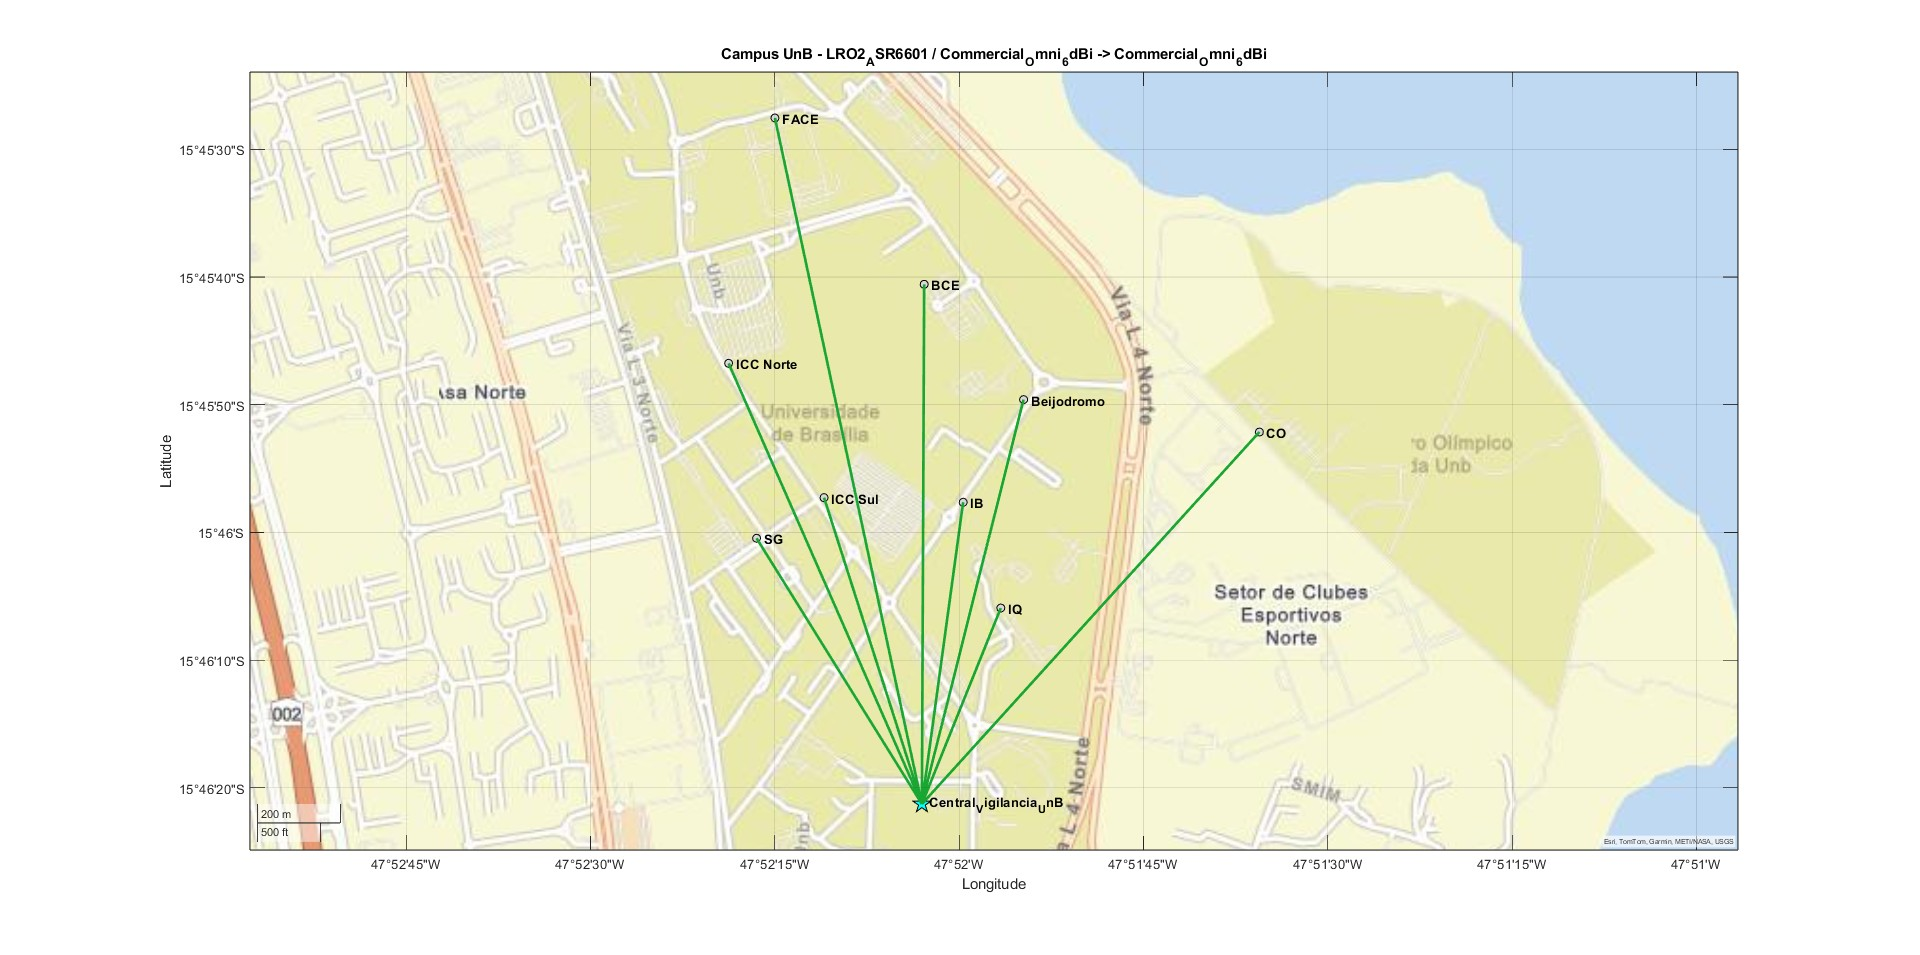
\includegraphics[width=\linewidth,height=0.68\textheight,keepaspectratio]{CampusUnBArranjoMapaSatelite.jpg}
\techcaption{Os enlaces convergem para a central/gateway. Como os azimutes são diferentes, uma antena única muito diretiva no gateway cria regiões mal cobertas.}
\column{0.36\textwidth}
\small
\begin{block}{O que observar}
\begin{itemize}
  \item FACE é o ponto mais distante.
  \item IQ, IB, SG e ICC Sul são enlaces mais curtos.
  \item CO desloca a cobertura para outro azimute.
  \item O gateway central precisa receber de uma faixa angular ampla.
\end{itemize}
\end{block}
\end{columns}
\end{frame}

% 32
\begin{frame}{Cenários simulados}
\small
\begin{table}
\centering
\scriptsize
\begin{tabular}{p{0.18\linewidth}p{0.72\linewidth}}
\toprule
Cenário & Objetivo \\
\midrule
A & Mesma antena no transmissor e no gateway. \\
B & Gateway omnidirecional vertical e transmissores variando entre antenas. \\
C & Transmissores diretivos apontados para o gateway e gateway omnidirecional. \\
D & Transmissores diretivos com erro de apontamento. \\
E & Comparação entre RFM95W, LRO2 ASR6601 e E220-900T22D. \\
P & Parabólicas de 30, 40, 50 e \SI{60}{cm} com ganho WebPRAC por ângulo. \\
\bottomrule
\end{tabular}
\end{table}
\begin{block}{Metodologia computacional}
Para cada combinação, a simulação calcula geometria, ganho efetivo, FSPL, potência recebida, margem, status e rankings de robustez/praticidade.
\end{block}
\end{frame}

% 33
\begin{frame}{Resultados agregados: combinação módulo-antena}
\small
\begin{table}
\centering
\scriptsize
\begin{tabular}{p{0.22\linewidth}p{0.24\linewidth}p{0.20\linewidth}rrr}
\toprule
Módulo & Antena TX & Antena GW & Margem mín. & Média & Score \\
\midrule
LRO2 ASR6601 & Comercial omni 6 dBi & Comercial omni 6 dBi & 56.78 & 61.74 & 98.61 \\
E220-900T22D & Comercial omni 6 dBi & Comercial omni 6 dBi & 55.78 & 60.74 & 97.36 \\
LRO2 ASR6601 & Comercial omni 6 dBi & Monopolo & 55.93 & 60.89 & 95.95 \\
LRO2 ASR6601 & Helicoidal apontada & Comercial omni 6 dBi & 58.78 & 63.74 & 94.16 \\
\bottomrule
\end{tabular}
\end{table}
\begin{block}{Leitura}
A helicoidal apontada pode ter margem alta, mas perde praticidade. O ranking agregado favorece a antena comercial omni por combinar margem, robustez e instalação simples.
\end{block}
\end{frame}

% 34
\begin{frame}{Erros de apontamento}
\small
\begin{columns}[T,onlytextwidth]
\column{0.48\textwidth}
\begin{table}
\centering
\begin{tabular}{rr}
\toprule
Erro angular & Queda média de margem \\
\midrule
2$^\circ$ & 0.02 dB \\
5$^\circ$ & 0.11 dB \\
10$^\circ$ & 0.46 dB \\
\bottomrule
\end{tabular}
\end{table}
\column{0.48\textwidth}
\begin{block}{Interpretação}
Nos casos simulados, a queda média indicada para a parabólica transmissora é pequena para esses erros, mas o risco de campo permanece: suporte, vibração, vento, desalinhamento acumulado e obstruções podem degradar o ganho efetivo.
\end{block}
\end{columns}
\begin{block}{Mensagem}
Antenas diretivas exigem projeto mecânico junto com projeto eletromagnético.
\end{block}
\end{frame}

% 35
\begin{frame}{Por que a parabólica não é a melhor solução geral}
\small
\begin{columns}[T,onlytextwidth]
\column{0.52\textwidth}
\begin{block}{Boa quando}
\begin{itemize}
  \item O enlace é fixo e ponto-a-ponto.
  \item O nó pode ser apontado para o gateway.
  \item A margem extra compensa suporte e manutenção.
  \item D = 50 ou \SI{60}{cm} é fisicamente aceitável.
\end{itemize}
\end{block}
\column{0.44\textwidth}
\begin{block}{Ruim quando}
\begin{itemize}
  \item Uma antena única deve receber vários azimutes.
  \item O ponto está sujeito a vento ou desalinhamento.
  \item O custo mecânico supera a melhoria de margem.
  \item A instalação precisa ser simples e replicável.
\end{itemize}
\end{block}
\end{columns}
\begin{block}{Comparação-chave}
Omni 6 dBi: margem mínima 55.78 dB e média 61.08 dB. Parabólica PRAC apontada: margem mínima 54.76 dB e média 63.30 dB. A diferença de média não elimina o custo de diretividade.
\end{block}
\end{frame}

% 36
\begin{frame}{Discussão de engenharia}
\small
\begin{table}
\centering
\scriptsize
\begin{tabular}{p{0.23\linewidth}p{0.33\linewidth}p{0.33\linewidth}}
\toprule
Critério & Favorece omni/monopolo/dipolo & Favorece diretivas \\
\midrule
Cobertura multi-azimute & Gateway central único & Enlace fixo específico \\
Margem máxima & Suficiente em muitos cenários & Maior no boresight \\
Instalação & Simples, leve, repetível & Exige apontamento e suporte \\
Manutenção & Menor sensibilidade a desalinhamento & Maior inspeção mecânica \\
Custo total & Menor integração mecânica & Pode subir com mastro/suporte \\
Flexibilidade & Aceita novos pontos em vários azimutes & Depende de nova orientação \\
\bottomrule
\end{tabular}
\end{table}
\begin{block}{Síntese}
O projeto não busca a antena de maior ganho absoluto; busca a solução mais coerente com operação, infraestrutura e geometria do campus.
\end{block}
\end{frame}

% 37
\begin{frame}{Escolha mais coerente para o gateway}
\small
\begin{block}{Recomendação técnica}
Para um gateway central único associado à infraestrutura já existente da segurança da UnB, a escolha mais coerente é uma antena omnidirecional vertical prática, com a comercial de \SI{6}{dBi} como referência forte.
\end{block}
\begin{columns}[T,onlytextwidth]
\column{0.48\textwidth}
\begin{itemize}
  \item Recebe de vários azimutes.
  \item Instalação mais simples.
  \item Boa margem simulada.
  \item Compatível com central já instalada.
\end{itemize}
\column{0.48\textwidth}
\begin{itemize}
  \item Evita apontamento único.
  \item Reduz complexidade mecânica.
  \item Facilita expansão do sistema.
  \item Setorização pode ser estudada se a cobertura exigir.
\end{itemize}
\end{columns}
\end{frame}

% 38
\begin{frame}{Escolha mais coerente para os nós de alarme}
\small
\begin{columns}[T,onlytextwidth]
\column{0.50\textwidth}
\begin{block}{Opção padrão}
\begin{itemize}
  \item Antena comercial omni 6 dBi ou monopolo vertical.
  \item Boa margem e instalação simples.
  \item Cobertura robusta mesmo com pequenas variações de montagem.
\end{itemize}
\end{block}
\column{0.46\textwidth}
\begin{block}{Casos especiais}
\begin{itemize}
  \item PCB compacta quando integração e custo dominam.
  \item Helicoidal ou parabólica em enlace fixo apontado.
  \item Parabólica apenas se suporte, alinhamento e manutenção forem aceitáveis.
\end{itemize}
\end{block}
\end{columns}
\begin{block}{Decisão por papel}
Gateway precisa de cobertura. Nó de alarme precisa de confiabilidade, baixo custo e instalação repetível; ganho diretivo só se justifica em pontos críticos.
\end{block}
\end{frame}

% 39
\begin{frame}{Implicações para implantação no campus}
\small
\begin{columns}[T,onlytextwidth]
\column{0.48\textwidth}
\begin{block}{Antes do piloto}
\begin{itemize}
  \item Medir ruído e ocupação espectral em 915 MHz.
  \item Validar altura de instalação e obstruções.
  \item Conferir $S_{11}$ e casamento das antenas reais.
  \item Definir proteção mecânica e elétrica.
\end{itemize}
\end{block}
\column{0.48\textwidth}
\begin{block}{Durante o piloto}
\begin{itemize}
  \item Registrar RSSI/SNR por ponto.
  \item Comparar margem simulada e campo.
  \item Testar mensagens de alarme e supervisão.
  \item Ajustar potência e espalhamento LoRa conforme consumo e confiabilidade.
\end{itemize}
\end{block}
\end{columns}
\end{frame}

% 40
\begin{frame}{Implicações para implantação no campus}
\small
\begin{columns}[T,onlytextwidth]
\column{0.48\textwidth}
\begin{block}{Antes do piloto}
\begin{itemize}
  \item Medir ruído e ocupação espectral em 915 MHz.
  \item Validar altura de instalação e obstruções.
  \item Conferir $S_{11}$ e casamento das antenas reais.
  \item Definir proteção mecânica e elétrica.
\end{itemize}
\end{block}
\column{0.48\textwidth}
\begin{block}{Durante o piloto}
\begin{itemize}
  \item Registrar RSSI/SNR por ponto.
  \item Comparar margem simulada e campo.
  \item Testar mensagens de alarme e supervisão.
  \item Ajustar potência e espalhamento LoRa conforme consumo e confiabilidade.
\end{itemize}
\end{block}
\end{columns}
\end{frame}

% ============================================================
% PARTE 3 — PLATAFORMA COMPUTACIONAL WEB
% ============================================================

% 41
\begin{frame}{Plataforma Web: visão geral}
\small
\begin{columns}[T,onlytextwidth]
\column{0.54\textwidth}
\begin{block}{Três módulos principais}
\begin{enumerate}
  \item \textbf{Sandbox} — criar e pré-visualizar antenas por tipo; simulação rápida com ganho, impedância, SWR e diagrama de radiação.
  \item \textbf{Biblioteca} — salvar, importar e exportar antenas como JSON; campos físicos persistidos.
  \item \textbf{Link Planner} — montar cenários com nós geográficos; calcular distância 3D, FSPL e margem de enlace com semáforo de viabilidade.
\end{enumerate}
\end{block}
\column{0.42\textwidth}
\begin{block}{Tecnologia}
\begin{itemize}
  \item Backend: \textbf{FastAPI} + \textbf{Pydantic}.
  \item Frontend: \textbf{HTML/CSS/JS} puro.
  \item Dados: arquivos \textbf{JSON} auditáveis.
  \item Deploy: \textbf{Docker} (imagem pública no Hub).
\end{itemize}
\end{block}
\end{columns}
\end{frame}

% 42
\begin{frame}{Sandbox — criação e visualização de antenas}
\begin{columns}[T,onlytextwidth]
\column{0.50\textwidth}
\centering
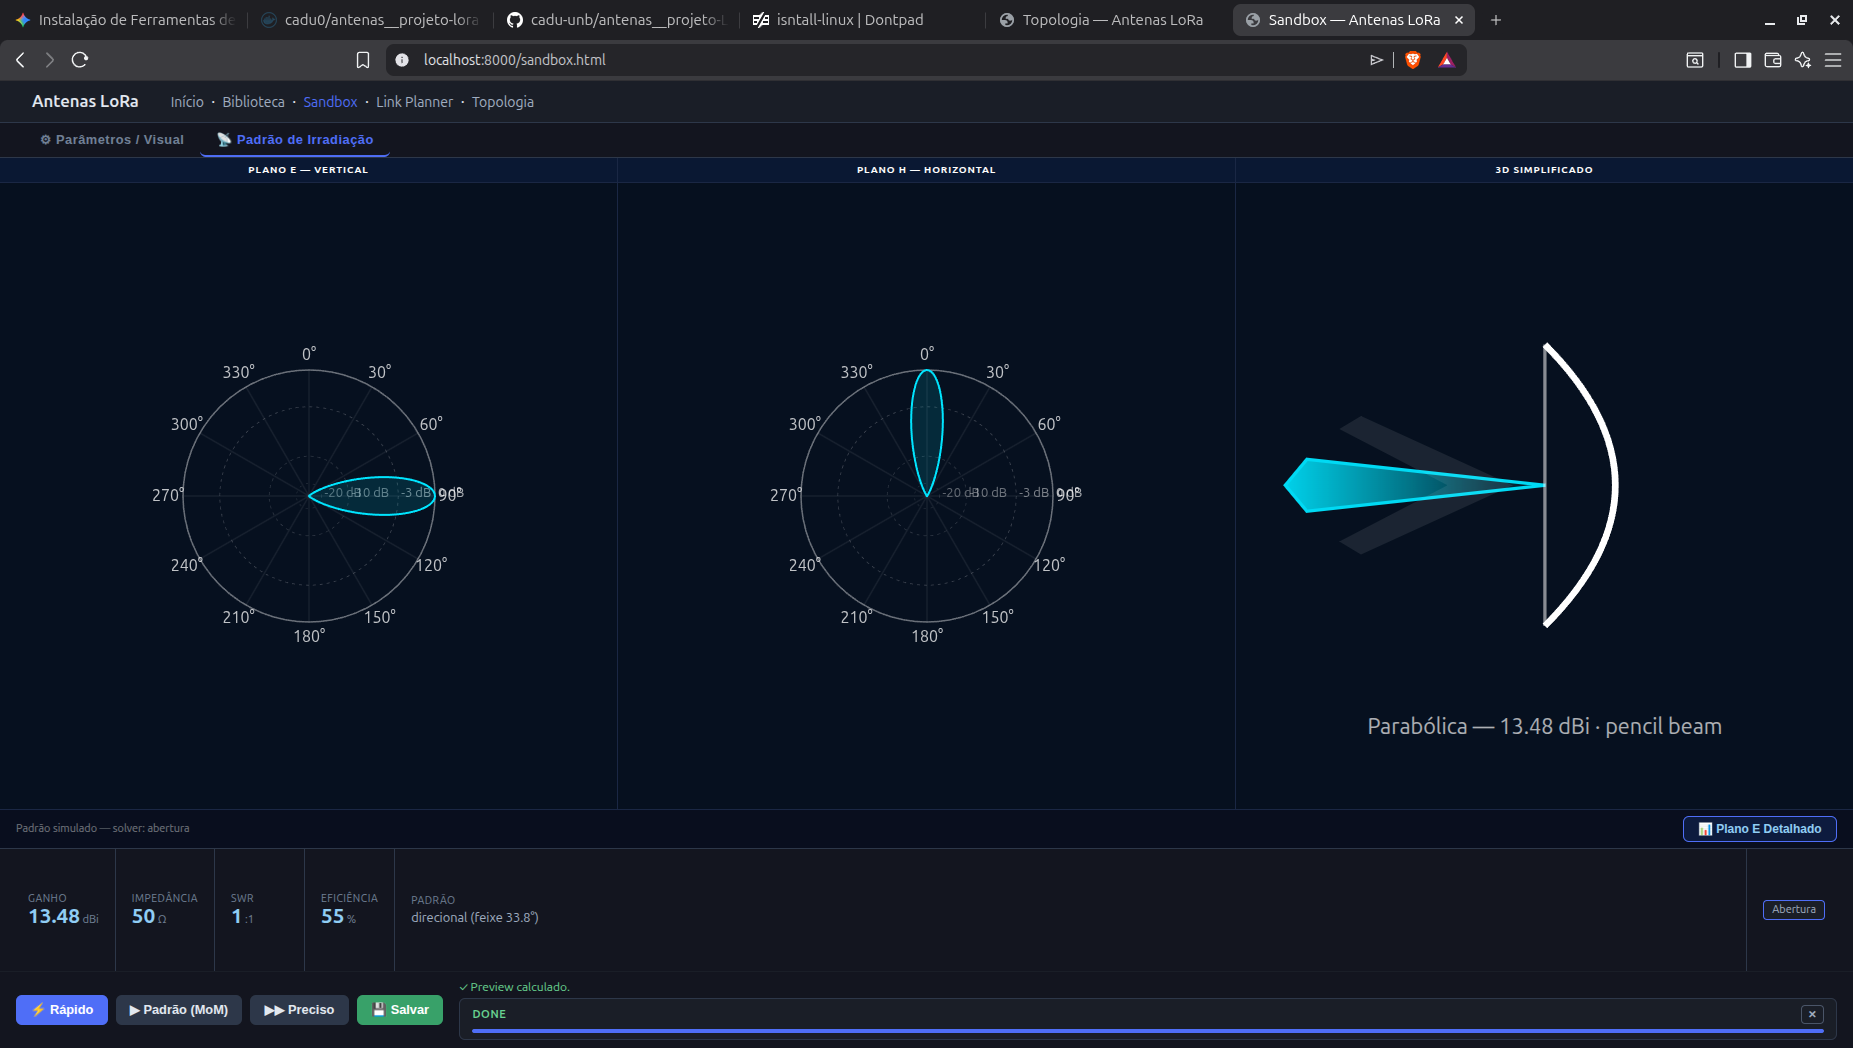
\includegraphics[width=\linewidth,height=0.60\textheight,keepaspectratio]{sandbox-visual.png}
\techcaption{Visualização gráfica da antena selecionada: padrão de radiação simplificado e geometria.}
\column{0.46\textwidth}
\centering
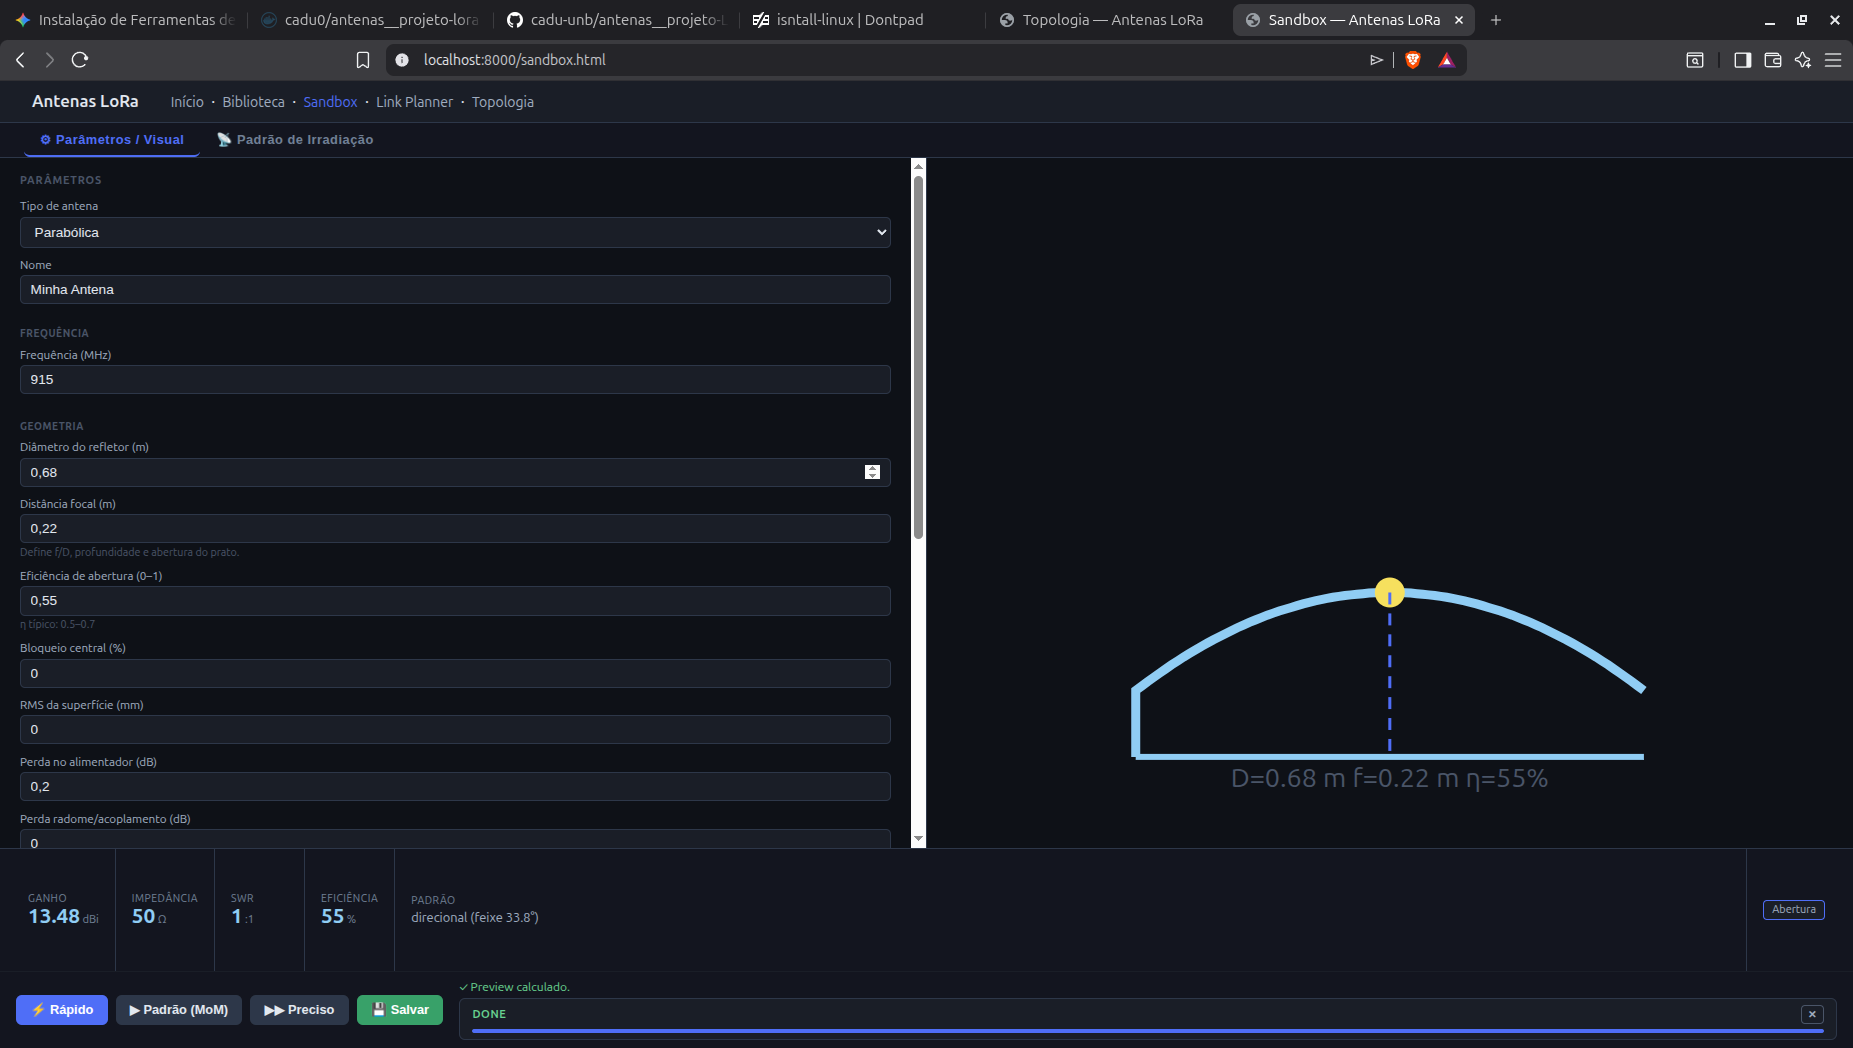
\includegraphics[width=\linewidth,height=0.60\textheight,keepaspectratio]{sandbox-parametros.png}
\techcaption{Parâmetros configuráveis e resultados: ganho, impedância, SWR, eficiência e campos físicos pré-preenchidos por tipo.}
\end{columns}
\end{frame}

% 43
\begin{frame}{Biblioteca de Antenas}
\begin{columns}[T,onlytextwidth]
\column{0.62\textwidth}
\centering
\vspace{-0.8cm}
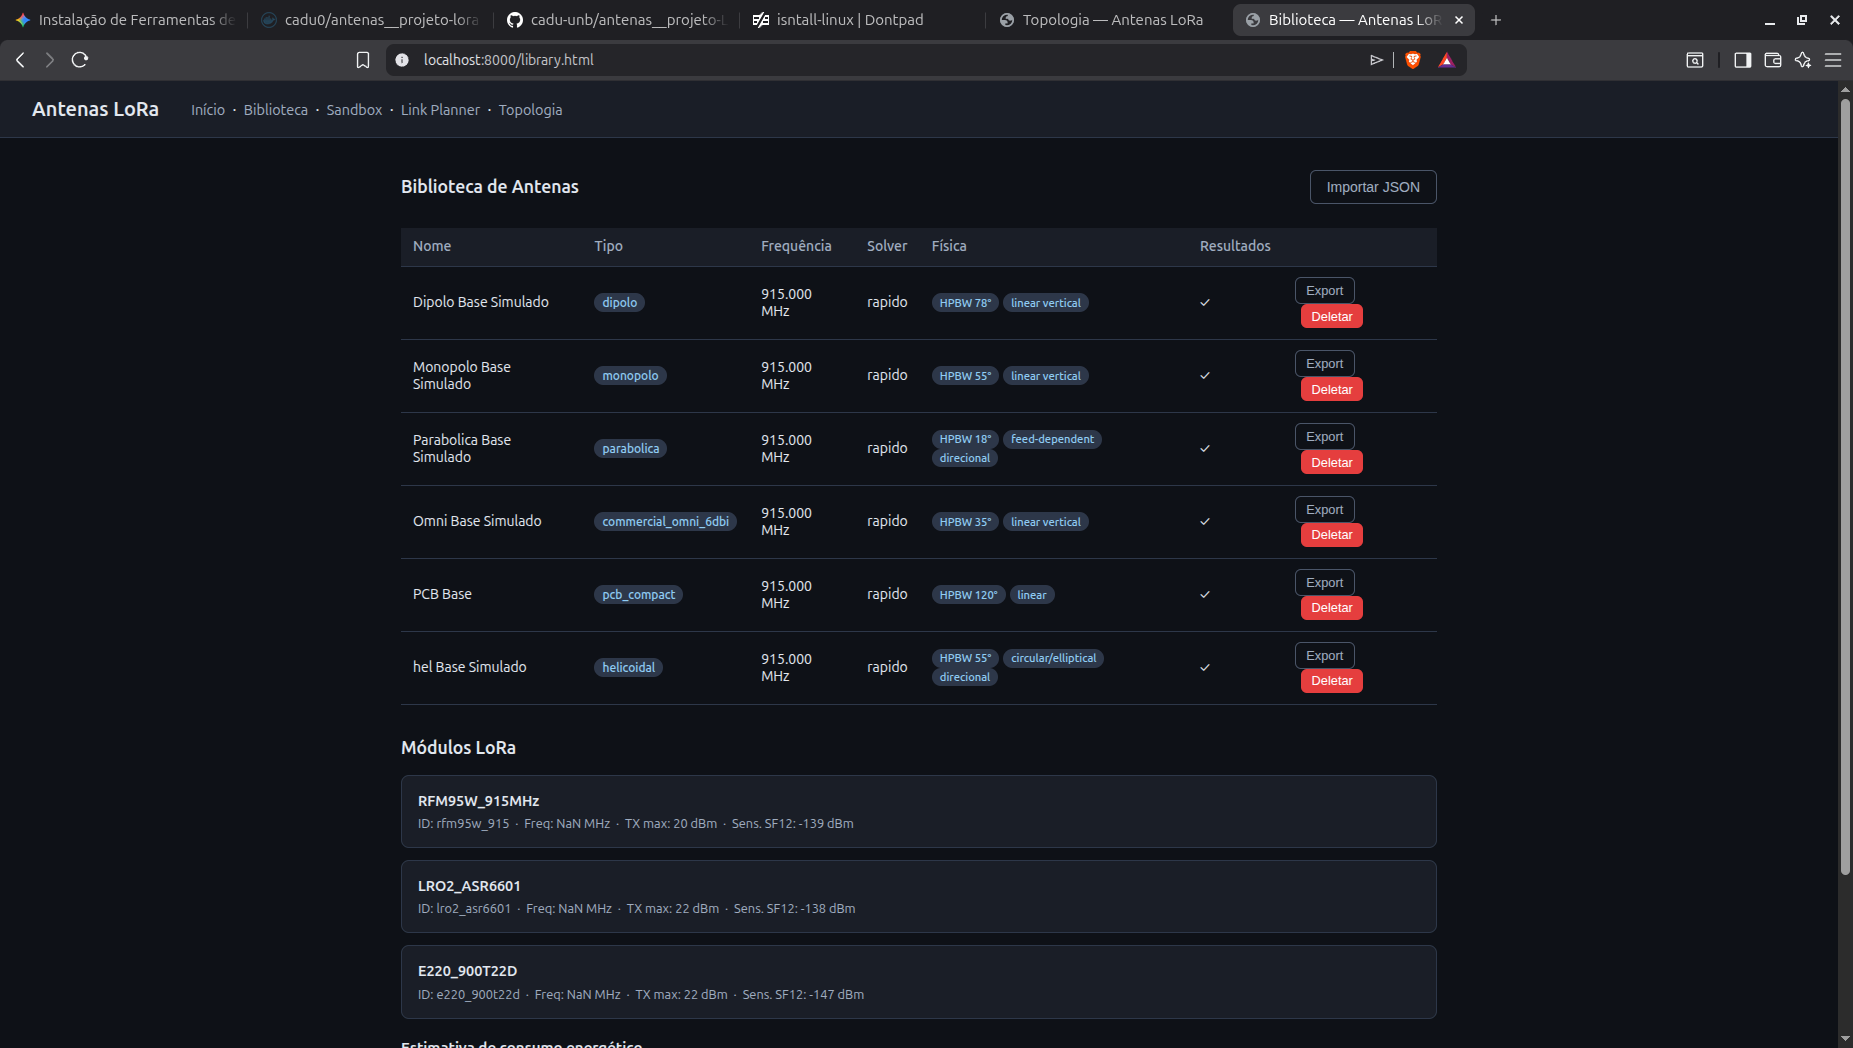
\includegraphics[width=\linewidth,height=0.68\textheight,keepaspectratio]{biblioteca-de-antenas.png}
\techcaption{A biblioteca lista antenas salvas com campos físicos — HPBW, polarização, direcionalidade — e permite exportar o JSON completo de cada especificação.}
\column{0.34\textwidth}
\small
\begin{block}{Fluxo}
\begin{enumerate}
  \item Criar antena no Sandbox.
  \item Salvar na Biblioteca.
  \item Exportar JSON ou reutilizar no Link Planner.
  \item Importar especificações de terceiros.
\end{enumerate}
\end{block}
\begin{block}{Schema}
Antenas v2.0 incluem \texttt{gmax\_dbi}, \texttt{hpbw\_deg}, polarização e scores de praticidade e multidireção.
\end{block}
\end{columns}
\end{frame}

% 44
\begin{frame}{Link Planner — cálculo de margem de enlace}
\begin{columns}[T,onlytextwidth]
\column{0.60\textwidth}
\centering
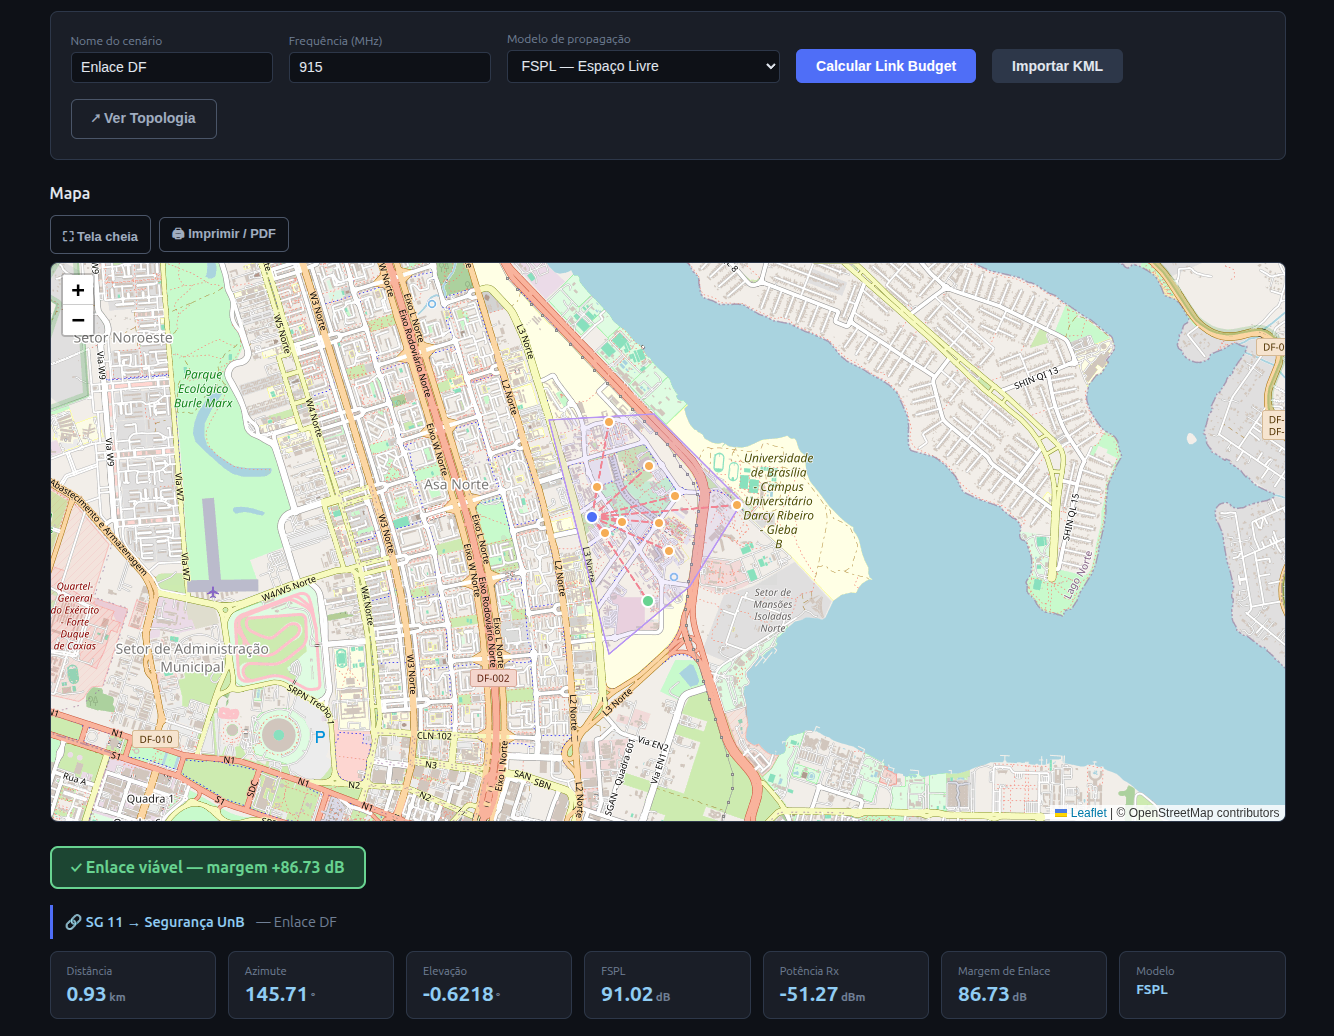
\includegraphics[width=\linewidth,height=0.75\textheight,keepaspectratio]{link-planer.png}
\column{0.36\textwidth}
\vspace{-1.2em}
\small
\begin{block}{Cálculo}
\begin{itemize}
  \item Distância 3D via ENU.
  \item FSPL em 915 MHz.
  \item Ganho efetivo direcional.
  \item Perdas adicionais e fading.
  \item Perda de polarização automática.
  \item Margem $M = P_{rx} - S_{rx}$.
\end{itemize}
\end{block}
\begin{block}{O que ver}
Nós com coordenadas reais, antenas da Biblioteca, semáforo de viabilidade e tabela de margem por enlace.
\end{block}
\end{columns}
\end{frame}

% 45
\begin{frame}{Topologia do sistema}
\begin{columns}[T,onlytextwidth]
\column{0.49\textwidth}
\centering
% topologia-segurança.png: nome com caracter especial — compilar com pdflatex UTF-8
% se der erro, renomear o arquivo para topologia-seguranca.png e ajustar aqui
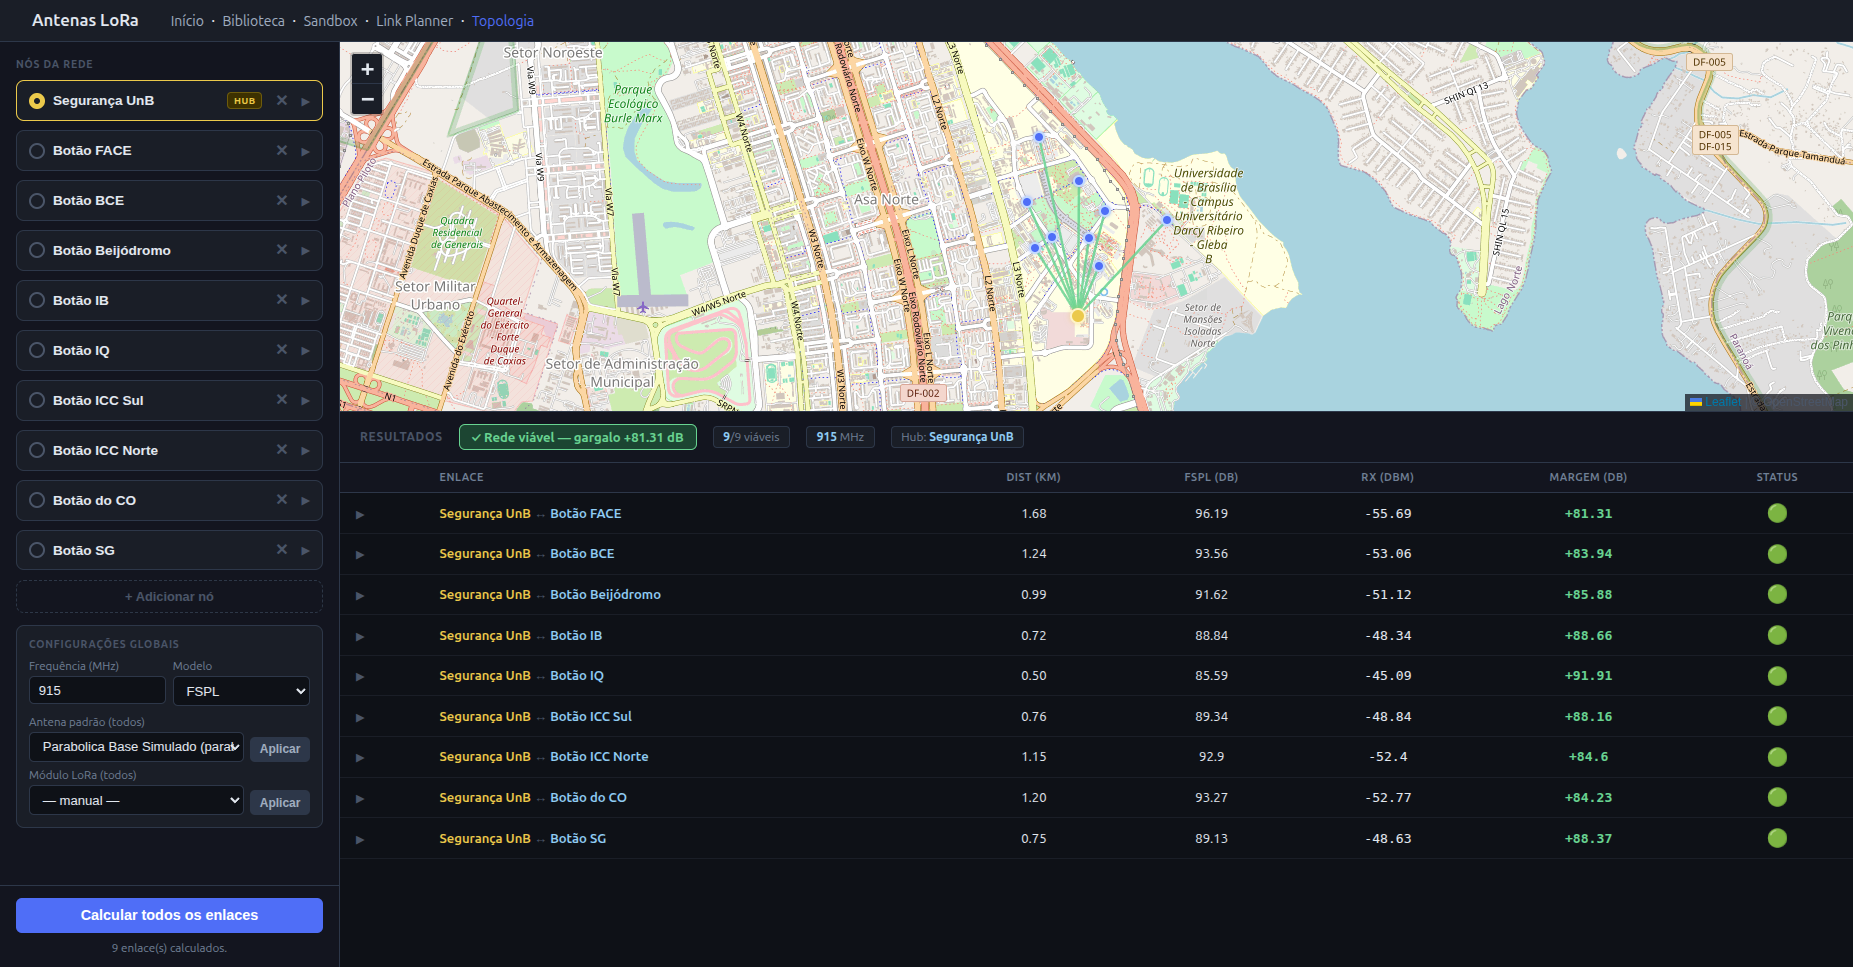
\includegraphics[width=\linewidth,height=0.62\textheight,keepaspectratio]{topologia-segurança.png}
\techcaption{Visão topológica do sistema de segurança: nós de alarme e gateway em estrela.}
\column{0.47\textwidth}
\centering
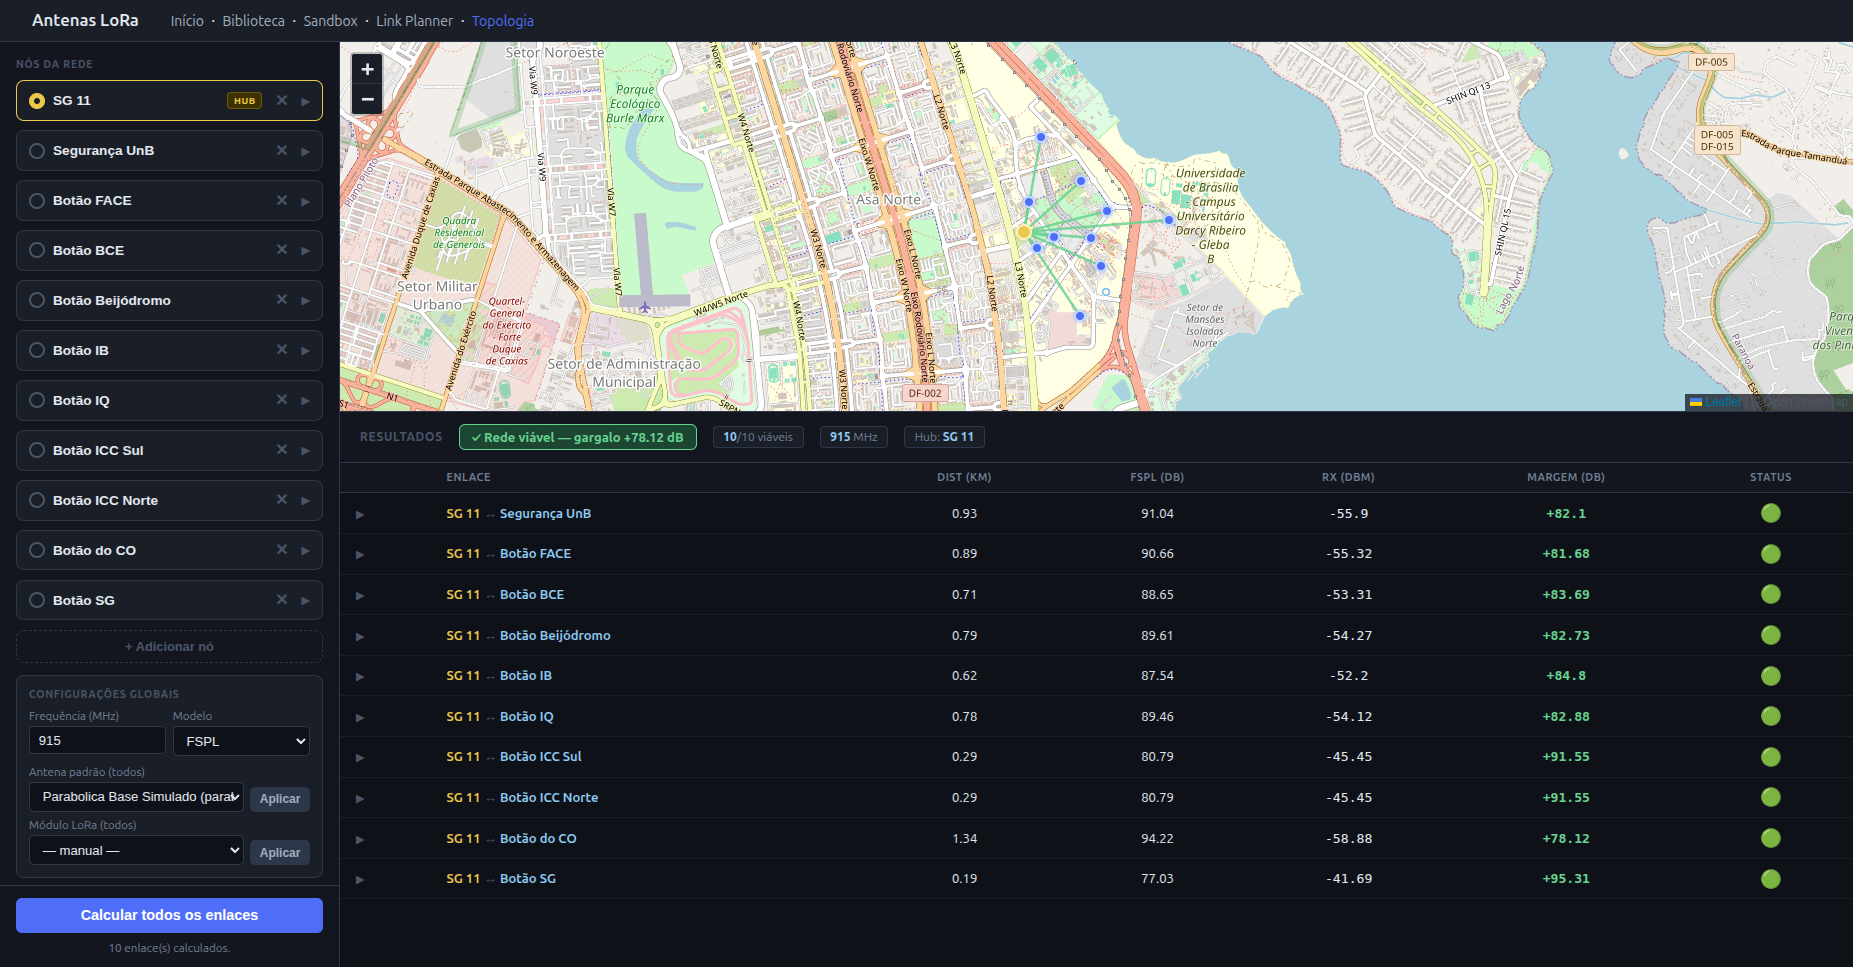
\includegraphics[width=\linewidth,height=0.62\textheight,keepaspectratio]{topologia-sg11.png}
\techcaption{Cenário detalhado com o ponto SG-11: enlace individual configurado e margem calculada.}
\end{columns}
\end{frame}

% 46
\begin{frame}{Projeto disponível publicamente}
\small
\begin{block}{Imagem Docker — deploy em um comando}
\url{https://hub.docker.com/repository/docker/cadu0/antenas__projeto-lora/general}

\vspace{0.5em}
\texttt{docker run -p 8000:8000 cadu0/antenas\_\_projeto-lora}
\end{block}
\begin{block}{Código-fonte}
\url{https://github.com/cadu-unb/antenas__projeto-LoRa.git}

\vspace{0.5em}
\begin{itemize}
  \item Backend FastAPI, schemas Pydantic, solvers de antena.
  \item Frontend HTML/CSS/JS — Sandbox, Biblioteca, Link Planner, Topologia.
  \item Scripts de backfill e suite de testes (\texttt{uv run pytest}).
  \item Documentação técnica em \texttt{docs/}.
\end{itemize}
\end{block}
\begin{block}{}
\centering
A plataforma está pronta para uso educacional, piloto e extensão por outros grupos da UnB.
\end{block}
\end{frame}

% ============================================================
% CONCLUSÃO E REFERÊNCIAS
% ============================================================

% 47
\begin{frame}{Conclusão}
\vspace{-.75cm}
\small
\begin{columns}[T,onlytextwidth]
\column{0.48\textwidth}
\begin{block}{O que o projeto mostrou}
\begin{itemize}
  \item Enlace LoRa é tecnicamente viável para emergências no campus — margens acima de 48 dB mesmo no ponto mais distante.
  \item A antena omnidirecional comercial de 6 dBi liderou o ranking agregado por combinar margem suficiente, cobertura em múltiplos azimutes e instalação simples.
  \item Antenas diretivas melhoram margem no boresight, mas exigem alinhamento e perdem em robustez para gateway central.
\end{itemize}
\end{block}
\column{0.48\textwidth}
\begin{block}{Contribuições}
\begin{itemize}
  \item Modelagem geométrica com coordenadas reais do Campus Darcy Ribeiro.
  \item Simulação comparativa de 6 antenas e 3 módulos LoRa em múltiplos cenários.
  \item Plataforma Web educacional com Sandbox, Biblioteca e Link Planner — disponível publicamente via Docker e GitHub.
\end{itemize}
\end{block}
\end{columns}
\begin{block}{Próximo passo}
Validação de campo: medir RSSI/SNR nos pontos reais e comparar com as margens simuladas.
\end{block}
\end{frame}

% 48
\begin{frame}{Referências}
\small
\begin{thebibliography}{9}

\bibitem{balanis2005}
BALANIS, Constantine A.
\textit{Antenna Theory: Analysis and Design}.
3.~ed. Hoboken: John Wiley \& Sons, 2005.

\bibitem{lavric2017}
LAVRIC, Alexandru; POPA, Valentin.
Internet of Things and LoRa\texttrademark{} Low-Power Wide-Area Networks: A Survey.
In: \textit{2017 International Symposium on Signals, Circuits and Systems (ISSCS)}.
IEEE, 2017.

\bibitem{terada}
TERADA, Marco Antonio Brasil.
\textit{Material de aula — Antenas e Propagação}.
Universidade de Brasília, Departamento de Engenharia Elétrica.

\end{thebibliography}
\end{frame}

\end{document}
